\documentclass[12pt]{article}\usepackage[]{graphicx}\usepackage[dvipsnames]{xcolor}
% maxwidth is the original width if it is less than linewidth
% otherwise use linewidth (to make sure the graphics do not exceed the margin)
\makeatletter
\def\maxwidth{ %
  \ifdim\Gin@nat@width>\linewidth
    \linewidth
  \else
    \Gin@nat@width
  \fi
}
\makeatother

\definecolor{fgcolor}{rgb}{0.345, 0.345, 0.345}
\newcommand{\hlnum}[1]{\textcolor[rgb]{0.686,0.059,0.569}{#1}}%
\newcommand{\hlstr}[1]{\textcolor[rgb]{0.192,0.494,0.8}{#1}}%
\newcommand{\hlcom}[1]{\textcolor[rgb]{0.678,0.584,0.686}{\textit{#1}}}%
\newcommand{\hlopt}[1]{\textcolor[rgb]{0,0,0}{#1}}%
\newcommand{\hlstd}[1]{\textcolor[rgb]{0.345,0.345,0.345}{#1}}%
\newcommand{\hlkwa}[1]{\textcolor[rgb]{0.161,0.373,0.58}{\textbf{#1}}}%
\newcommand{\hlkwb}[1]{\textcolor[rgb]{0.69,0.353,0.396}{#1}}%
\newcommand{\hlkwc}[1]{\textcolor[rgb]{0.333,0.667,0.333}{#1}}%
\newcommand{\hlkwd}[1]{\textcolor[rgb]{0.737,0.353,0.396}{\textbf{#1}}}%
\let\hlipl\hlkwb

\usepackage{framed}
\makeatletter
\newenvironment{kframe}{%
 \def\at@end@of@kframe{}%
 \ifinner\ifhmode%
  \def\at@end@of@kframe{\end{minipage}}%
  \begin{minipage}{\columnwidth}%
 \fi\fi%
 \def\FrameCommand##1{\hskip\@totalleftmargin \hskip-\fboxsep
 \colorbox{shadecolor}{##1}\hskip-\fboxsep
     % There is no \\@totalrightmargin, so:
     \hskip-\linewidth \hskip-\@totalleftmargin \hskip\columnwidth}%
 \MakeFramed {\advance\hsize-\width
   \@totalleftmargin\z@ \linewidth\hsize
   \@setminipage}}%
 {\par\unskip\endMakeFramed%
 \at@end@of@kframe}
\makeatother

\definecolor{shadecolor}{rgb}{.97, .97, .97}
\definecolor{messagecolor}{rgb}{0, 0, 0}
\definecolor{warningcolor}{rgb}{1, 0, 1}
\definecolor{errorcolor}{rgb}{1, 0, 0}
\newenvironment{knitrout}{}{} % an empty environment to be redefined in TeX

%\usepackage{alltt}
\usepackage{amsmath,amsfonts,amssymb,graphicx,authblk}
\usepackage[font={footnotesize,singlespacing},labelfont=bf]{caption}
\usepackage{titlesec,blkarray, bm} 
\usepackage{float,afterpage}
\usepackage[running,mathlines]{lineno}
\usepackage[vmargin=1in,hmargin=1in]{geometry}
\usepackage[authoryear,sort]{natbib}
\usepackage[dvipsnames]{xcolor}
\usepackage[nodisplayskipstretch]{setspace} 
\usepackage[section]{placeins}
\usepackage{gensymb}
\usepackage{enumitem}
\usepackage{orcidlink}
\usepackage{tabularx} % put this once in your preamble
\usepackage{booktabs}
\usepackage{pdflscape}  % or \usepackage{lscape}
\usepackage{adjustbox}
\usepackage{newfloat}   % for creating new float types
\usepackage{tocloft}    % for customizing lists
\usepackage{caption}
\usepackage{rotating}
\usepackage{xr-hyper} % cross-references between main text and SI
\usepackage{hyperref}
\externaldocument{../Main_Manuscript/EcolLett_R2}
\usepackage{makecell} % 
\usepackage{longtable}
\usepackage{pdflscape}
\setlist{topsep=.125em,itemsep=-0.15em,leftmargin=0.75cm}
\setlength{\parindent}{0.35in}

\usepackage[sc]{mathpazo} %Like Palatino with extensive math support
\usepackage[subtle]{savetrees}

\usepackage{lineno}
%\renewcommand{\refname}{Literature Cited}
%\renewcommand{\floatpagefraction}{0.9}
%\renewcommand{\topfraction}{0.99}
%\renewcommand{\textfraction}{0.05}

\clubpenalty = 10000
\widowpenalty = 10000

\sloppy 

\usepackage{ifpdf}
\ifpdf
\DeclareGraphicsExtensions{.pdf,.png,.jpg}
\DeclareFloatingEnvironment[fileext=losf, listname={List of Supplementary Figures}]{suppfigure}
\DeclareFloatingEnvironment[fileext=lost, listname={List of Supplementary Tables}]{supptable}
\usepackage{epstopdf}
\else
\DeclareGraphicsExtensions{.eps}
\fi

%\graphicspath{{/Users/jacobmoutouama/Dropbox/Miller Lab/github/endo-range-limits/Manuscript/Ecology letters/Manuscript/LaTexR1/Figure}}
%\graphicspath{{C:/Users/tm9/Dropbox/github/ELVI-endophyte-density/Figure}}
\newcommand{\tom}[2]{{\color{red}{#1}}\footnote{\textit{\color{red}{#2}}}}
\newcommand{\jacob}[2]{{\color{blue}{#1}}\footnote{\textit{\color{blue}{#2}}}}
\renewcommand\Authfont{\normalfont\normalsize}    % sets author names to small
\renewcommand\Affilfont{\normalfont\small} % sets affiliations even smaller
\newcommand{\revise}[1]{{\color{Mahogany}{#1}}}
%\newcommand{\Sminus}{S\revise{\textminus{}}}
%\renewcommand{\thesuppfigure}{S\arabic{suppfigure}}
%\renewcommand{\thesupptable}{S\arabic{supptable}}
\setlength{\affilsep}{1em}  
%\doublespacing



% I cannot get \orcidlink working on my computer so for now replacing this with \textit

%-------------------------------------------------------------------------
\title{\Large Aridity and herbivory shape demographic benefits of fungal endophytes in cool-season grasses}
\author[1, 2]{Jacob K. Moutouama\,\orcidlink{0000-0003-1599-1671} \thanks{Corresponding author: jmoutouama@gmail.com}}
\author[3]{Joshua C. Fowler}
\author[4]{Akiem M. Gough}
\author[4]{Julia Martin}
\author[4]{Christopher C. Oxley}
\author[4]{Karl M. Schrader}
\author[4]{Karis Williams}
\author[4]{Tom E.X. Miller\,\orcidlink{0000-0003-3208-6067}}
\affil[1]{Department of Botany, University of British Columbia, Vancouver, BC, Canada}
\affil[2]{African Centre for DNA Barcoding, University of Johannesburg, Johannesburg, South Africa}
\affil[3]{Department of Environmental Studies, University of Colorado Boulder, Boulder, CO, USA}
\affil[4]{Department of BioSciences, Rice University, Houston, TX, USA}
\date{} % clear date


\sloppy

%-------------------------------------------------------------------------
\IfFileExists{upquote.sty}{\usepackage{upquote}}{}
\frenchspacing
\begin{document}
\renewcommand{\baselinestretch}{1.2}
\begin{center}
{\Large\textbf{Supporting Information}}\\[1em]
{\large Aridity and herbivory shape demographic benefits of fungal endophytes in cool-season grasses}\\[1em]
Jacob K. Moutouama, Joshua C. Fowler, Akiem M. Gough, Julia Martin, Christopher C. Oxley, Karl M. Schrader, Karis Williams, and Tom E.X. Miller
\end{center}
\linenumbers
\spacing{1.25}


% --- Reset counters ---
\setcounter{figure}{0}
\setcounter{table}{0}
\setcounter{equation}{0}
\setcounter{section}{0}

% --- Section numbering ---
\renewcommand{\thesection}{S.\arabic{section}}

% --- Equation numbering ---
\renewcommand{\theequation}{S\arabic{equation}}

% --- Figure numbering ---
\renewcommand{\figurename}{Fig}
\renewcommand{\thefigure}{S\arabic{figure}}

% --- Table numbering ---
\renewcommand{\thetable}{S\arabic{table}}
\renewcommand{\tablename}{Table}

\section {Supporting Information}
\subsection {Supporting Methods}
\subsubsection {Endophyte status verification}
To assess the efficacy of heat treatment and to confirm endophyte status before transfer to the field experiment, we verified symbiont status ($S^+$ or $S^-$) of plants from control and heat lineages using three methods. 
First, peels of the inner leaf sheaths were stained with aniline blue lactic acid and viewed under a compound microscope at 200$\times$--400$\times$ to identify \emph{Epichloë} hyphae \citep{jackson1988rapid}. 
Second, we used microscopy to assess the presence or absence of \emph{Epichloë} in seeds that were soaked in NaOH, then squashed and stained similarly to the leaf tissue, to determine the endophyte status of the maternal plant \citep{fowler2025increasing}. 
Third, we used an immunoblot assay (Phytoscreen field tiller endophyte detection kit, Agrinostics Ltd. Co., Watkinsville, Georgia, USA) that targets proteins of \emph{Epichloë} spp. to visually indicate presence or absence \citep{koh2006rapid}. 
In total, we tested 1,481 plants for endophyte status. 
In cases where two or more methods were used on the same plants ($N=253$), there was 99.2\% agreement between methods.
For genotypes that were vegetatively propagated, we tested the endophyte status of a single clonal replicate and assumed that its status applied equally to all clones. 

All $S^-$ plants used in the experiment came from heat-treated lineages, while $S^+$ plants came from both control and heat lineages depending on the efficacy of the removal treatment. 
While heat treatment was effective at reducing endophyte prevalence relative to controls, our confidence that individual $S^-$ plants were experimentally disinfected, as opposed to naturally symbiont-free, varied due to among-population variation in endophyte prevalence (mean: 68\% $S^+$) and the effectiveness of the heat treatment (Table \ref{tab:heat_treatment}). 
For example, for the SJC population of \emph{A. hyemalis}, control and heat lineages yielded plants that were 100\% and 5\% $S^+$, respectively -- giving us high confidence that $S^-$ plants are derived from successful symbiont removal. 
For the SFAEF population of \emph{P. autumnalis}, on the other hand, control and heat lineages yielded plants that were 35\% and 26\% $S^+$, respectively -- meaning that these $S^-$ plants were quite likely from naturally $S^-$ lineages.


\subsection{Greenhouse experiment}
\label{sec:greenhouse}

\subsubsection{Experimental design}

To examine whether edaphic factors mediate plant performance across the precipitation gradient, we conducted a greenhouse experiment
manipulating soil origin and endophyte status.
Soils were collected during summer 2024 from the seven field sites used in the common garden experiment.
These sites span the precipitation gradient from the wettest site to the driest site. 
After collection, soils were stored in a cold room at 3.3°C until the start of the experiment. 
Soils were not sterilized and therefore soil origin treatment reflects both the physical properties of the soil as well as the microbial communities that may vary across soil types.

Seeds of \textit{Agrostis hyemalis} were obtained from the seed stock used to generate plants in the range-limits field experiment. 
Seeds originated from two source populations (LPEF and SJC) and were grouped according to endophyte status as endophyte-symbiotic ($S^+$) or endophyte-free ($S^-$).
Seeds were germinated on agar plates (18.2 g agar per 1000 mL deionized water) in a growth chamber and subsequently transplanted as seedlings
into pots containing soils from each field site. 
Plants were randomly assigned to greenhouse trays and maintained under controlled greenhouse conditions with automated irrigation.
The experimental design crossed seed source population, endophyte status, and soil origin. 
Realised sample sizes varied across treatment combinations due to mortality and poor germination and are reported in Table~\ref{tab:soil_pop}.

\subsubsection {Data collection}

Plants were monitored regularly for survival and reproductive development. 
Reproductive output was quantified as inflorescence number.
During the flowering season, plants were checked at least twice per week for the presence of seed-bearing inflorescences. 
Mature inflorescences were collected and counted as they developed to avoid repeated counts. 
After eight months of growth, plants were harvested to quantify aboveground biomass. 
Plant material was dried at 60\textdegree C in a drying oven and weighed using an analytical balance. 
Because inflorescences were collected prior to harvest, they were dried separately and added to the total aboveground biomass.

\subsubsection {Statistical analysis}
\phantomsection
\addcontentsline{toc}{subsubsection}{Statistical analysis}
\label{sec:greenhouse_models}
For each fitness component (aboveground biomass and inflorescence count), we fitted hierarchical Bayesian models mirroring the field analysis. Fixed effects included symbiont status 
($S^+$/$S^-$), the 30-year mean annual precipitation of each soil's origin site (standardized; hereafter soil-origin MAP), and their interaction, with planting date (standardized) as a covariate. 
Source population was included as a random effect with a non-centered parameterization. 
Biomass was log-transformed and modeled with a Student-t likelihood ($\nu = 3$) to provide robustness to outliers, which are common in small greenhouse experiments; inflorescence count was modeled with a negative binomial likelihood to accommodate overdispersion. 
For all models, fixed-effect coefficients received $\text{Normal}(0, 1)$ priors; the overdispersion parameter for the inflorescence model was placed on the log scale with a $\text{Normal}(2, 1)$ prior (centered on $\phi \approx 7$); and the random-effect standard deviation received an $\text{Exponential}(2)$ prior.

Models were fitted in Stan \citep{Rstan} with four chains of 2,000 iterations (1,000 warmup; adapt\_delta $= 0.99$). Convergence was assessed via $\hat{R} < 1.01$ for all parameters and inspection of trace plots.
We report posterior medians with 95\% credible intervals for three focal parameters: the symbiont main effect ($S^+$ vs.\ $S^-$ at mean soil-origin MAP), the soil-origin MAP main effect, and the symbiont $\times$ soil-origin MAP interaction. 
To visualize how the endophyte effect varies across the soil-origin precipitation gradient, we computed the posterior contrast ($S^+ - S^-$) 
at each point along the observed precipitation range, marginalizing over planting date (set to the mean) and source population random effects. 
These contrasts are summarized as posterior medians with 95\% credible intervals and displayed alongside the predicted responses for each symbiont status. 
Posterior predictive checks indicated adequate fit for both models (Fig.~\ref{sup:ppc_models_soil}).
\clearpage



\begin{landscape}
\subsection*{Supporting Tables}
\begin{table}[htbp]
    \centering
     \caption{Geographic coordinates and descriptions of source populations for study species. For each source population, the table shows the total number of plants included in the experiment, the number of unique genotypes, and the average clonal replication per genotype.}
    \small
    \begin{tabular}{@{}ll
                r r
                >{\raggedright\arraybackslash}p{4.4cm}
                r r r@{}}
  \hline
Species & Population & Latitude & Longitude & Notes &
  \shortstack[r]{Total\\plants} &
  \shortstack[r]{Unique\\genotypes} &
  \shortstack[r]{Mean clones\\per genotype} \\
  \hline
\textit{A. hyemalis}   & SJC   & 30.7720 & $-$95.2006 & Private property, San Jacinto County, TX & 273 & 201 & 1.36 \\
\textit{A. hyemalis}   & COHR  & 29.6728 & $-$96.5675 & Roadside collection, Columbus, TX & 289 & 35 & 8.26 \\
\textit{A. hyemalis}   & LPEF  & 30.0854 & $-$97.1725 & Stengl Lost Pines Field Station, Bastrop, TX & 278 & 41 & 6.78 \\
\textit{P. autumnalis} & LA7   & 30.8497 & $-$93.2768 & Roadside population, DeRidder, LA & 91 & 9 & 10.11 \\
\textit{P. autumnalis} & LA1   & 32.5681 & $-$93.9330 & Walter P. Jacobs Nature Center, Shreveport, LA & 129 & 7 & 18.43 \\
\textit{P. autumnalis} & LA2   & 31.1830 & $-$92.6170 & Kisatchie National Forest, LA & 253 & 15 & 16.87 \\
\textit{P. autumnalis} & SFAEF & 31.4922 & $-$94.7722 & Stephen F. Austin Experimental Forest, TX & 247 & 41 & 6.02 \\
\textit{E. virginicus} & HUNT  & 30.7418 & $-$95.4745 & Pineywoods Environmental Research Laboratory, Huntsville, TX & 91 & 61 & 1.49 \\
\textit{E. virginicus} & RL5   & 30.4717 & $-$99.7838 & Llano River Field Station, Junction, TX & 131 & 91 & 1.44 \\
\textit{E. virginicus} & PALM  & 29.5916 & $-$97.5848 & Palmetto State Park, TX & 442 & 195 & 2.27 \\
\textit{E. virginicus} & JLP   & 29.7851 & $-$90.1149 & Jean Lafitte Park, LA & 176 & 102 & 1.73 \\
  \hline
\end{tabular}
       \label{tab:source_pop}
\end{table}
\end{landscape}
\clearpage


\begin{table}[ht]
    \centering
    \caption{Summary of symbiont removal treatments by species and population.
    N indicates the number of plants tested for symbiont status and
    \%$S^+$ indicates the proportion that tested positive.
    Treatment refers to the symbiont removal treatment applied to the seed lineage: Control (no treatment) or Heat (5 days in a drying oven at 60\degree C for \emph{E. virginicus} and \emph{P. autumnalis}; 12 min in a 60\degree C water bath for \emph{A. hyemalis}).
    For all populations except SFAEF and PALM, heat-treated seed lineages were one or more generations removed from the treatment; for those two populations, plants from heat-treated seeds were used directly in the experiment.}
    \label{tab:heat_treatment}
    % latex table generated in R 4.4.2 by xtable 1.8-4 package
% Tue Feb 10 16:05:39 2026
\begin{tabular}{lllrr}
  \hline
Species & Population & Treatment & N & \%S+ \\ 
  \hline
\textit{A. hyemalis} & COHR & Control &  84 & 0.92 \\ 
  \textit{A. hyemalis} & COHR & Heat &  75 & 0.04 \\ 
  \textit{A. hyemalis} & LPEF & Control &   7 & 0.57 \\ 
  \textit{A. hyemalis} & LPEF & Heat &  88 & 0.00 \\ 
  \textit{A. hyemalis} & SJC & Control & 132 & 1.00 \\ 
  \textit{A. hyemalis} & SJC & Heat & 191 & 0.05 \\ 
  \textit{E. virginicus} & HUNT & Control &  71 & 0.61 \\ 
  \textit{E. virginicus} & HUNT & Heat &  38 & 0.21 \\ 
  \textit{E. virginicus} & JLP & Control &  27 & 1.00 \\ 
  \textit{E. virginicus} & JLP & Heat & 113 & 0.02 \\ 
  \textit{E. virginicus} & PALM & Control & 176 & 0.61 \\ 
  \textit{E. virginicus} & PALM & Heat & 238 & 0.71 \\ 
  \textit{E. virginicus} & RL5 & Control &  68 & 0.43 \\ 
  \textit{E. virginicus} & RL5 & Heat &  74 & 0.73 \\ 
  \textit{P. autumnalis} & LA1 & Control &   5 & 0.20 \\ 
  \textit{P. autumnalis} & LA1 & Heat &   4 & 0.00 \\ 
  \textit{P. autumnalis} & LA2 & Control &  10 & 0.80 \\ 
  \textit{P. autumnalis} & LA2 & Heat &   3 & 0.33 \\ 
  \textit{P. autumnalis} & LA7 & Control &   5 & 1.00 \\ 
  \textit{P. autumnalis} & LA7 & Heat &  11 & 0.00 \\ 
  \textit{P. autumnalis} & SFAEF & Control &  23 & 0.35 \\ 
  \textit{P. autumnalis} & SFAEF & Heat &  38 & 0.26 \\ 
   \hline
\end{tabular}

\end{table}
\clearpage

\begin{table}[ht]
\caption{Common garden sites used in the field experiment, ordered from west to east.}
\label{tab:exp_sites}
\begin{tabular}{llrr}
\hline
Site & Code & Latitude & Longitude \\
\hline
TAMU Sonora Station                              & SON & 30.273467 & -100.561463 \\
Private property, Kerrville, TX                  & KER & 30.028437 & -99.142888 \\
Brackenridge Field Laboratory                    & BFL & 30.284866 & -97.780675 \\
UT Stengl Lost Pines Field Station               & BAS & 30.092343 & -97.172442 \\
TAMU Ecology and Natural Resource Teaching Area  & COL & 30.569302 & -96.366324 \\
Center for Biological Field Studies              & HUN & 30.742815 & -95.476881 \\
University of Louisiana Ecology Center           & LAF & 30.304773 & -92.012401 \\
\hline
\end{tabular}
\end{table}
\clearpage

\begin{table}[ht]
\centering
\caption{Comparison of candidate models (quadratic vs.\ linear) for each vital rate based on leave-one-out cross-validation (LOOCV).
$\Delta$ELPD is the difference in expected log pointwise predictive density relative to the best model.}
\label{tab:model_comparison}
\begin{tabular}{llrr}
\hline
Vital rate & Model type & $\Delta$ELPD & SE \\
\hline
Survival      & Linear    & 0.000  & 0.000 \\
Survival      & Quadratic & -0.282 & 0.663 \\
Growth        & Linear    & 0.000  & 0.000 \\
Growth        & Quadratic & -0.078 & 0.430 \\
Inflorescence & Linear    & 0.000  & 0.000 \\
Inflorescence & Quadratic & -0.689 & 0.516 \\
Spikelet      & Linear    & 0.000  & 0.000 \\
Spikelet      & Quadratic & -0.332 & 0.579 \\
\hline
\end{tabular}
\end{table}
\clearpage

\begin{table}[ht]
 \caption{Sample sizes for each combination of seed source population, soil-origin site, and endophyte treatment in the greenhouse experiment.
The experiment crossed two seed source populations (LPEF and SJC), seven soil-origin sites along the precipitation gradient, and two symbiont treatments ($S^-$ and $S^+$). Most treatment combinations included seven replicates, except LPEF $\times$ BFL $\times$ $S^-$ where $n = 6$ due to early mortality.}   
    \centering
    \small
    \begin{tabular}{llrr}
\hline
Response & Site & S- & S+ \\
\hline

\multicolumn{4}{l}{\textit{Biomass}} \\
 & LAF & 14 & 14 \\
 & SON & 14 & 14 \\
 & KER & 14 & 14 \\
 & BFL & 13 & 14 \\
 & BAS & 14 & 14 \\
 & COL & 14 & 14 \\
 & HUN & 14 & 14 \\
%\hline

\multicolumn{4}{l}{\textit{Inflorescence}} \\
 & LAF & 14 & 14 \\
 & SON & 14 & 14 \\
 & KER & 14 & 14 \\
 & BFL & 14 & 14 \\
 & BAS & 14 & 14 \\
 & COL & 14 & 14 \\
 & HUN & 14 & 14 \\
%\hline

\multicolumn{4}{l}{\textit{Spikelets}} \\
 & LAF &  7 & 10 \\
 & SON &  3 &  1 \\
 & KER &  1 &  0 \\
 & BFL &  3 &  8 \\
 & BAS &  7 &  6 \\
 & COL &  2 &  2 \\
 & HUN &  5 & 12 \\
\hline
\end{tabular}

    \label{tab:soil_pop}
\end{table}
\clearpage

% latex longtable (pivoted: Full data / Excl. KER-SON shown as paired columns)
% requires \usepackage{longtable}, \usepackage{pdflscape}, \usepackage{booktabs}
\begin{landscape}
% \small removed so font matches other supplementary tables
\setlength{\tabcolsep}{4pt}
\begin{longtable}{llllcccc}
\caption{Sensitivity of estimated endophyte effects to exclusion of sites KER and SON, which were destroyed by deer and subsequently replanted in 2024. For each combination of vital rate (Trait), species, herbivory treatment (Access = herbivory-access plots, Exclusion = herbivore-exclusion plots), and precipitation (Precip., in mm; three values spanning each species' observed precipitation range), the table reports the posterior median and 90\% credible interval [Med.\ $\Delta$ (90\% CI)] and the posterior probability of a positive endophyte effect [P($\Delta>0$)] for the full dataset and for the dataset excluding KER and SON. The endophyte effect $\Delta$ is defined as Pr(S+) $-$ Pr(S-) for survival, or the analogous difference on the response scale (S+ $-$ S-) for growth, inflorescence production, and spikelet production. Spikelet production was not modeled for \textit{A.\ hyemalis} because spikelets in this species were too numerous and small to count reliably (see Methods). Posterior estimates were nearly identical between the full dataset and the dataset excluding KER and SON across all species, vital rates, and herbivory treatments, indicating that the disturbance and replanting at these two sites did not meaningfully influence our conclusions.} \label{tab:sensitivity_KER_SON} \\
\toprule
& & & & \multicolumn{2}{c}{Full data} & \multicolumn{2}{c}{Excl.\ KER/SON} \\
\cmidrule(lr){5-6} \cmidrule(lr){7-8}
Trait & Species & Herbivory & Precip.\ (mm) & Med.\ $\Delta$ (90\% CI) & P($\Delta{>}0$) & Med.\ $\Delta$ (90\% CI) & P($\Delta{>}0$) \\
\midrule
\endfirsthead

\multicolumn{8}{c}{{\tablename\ \thetable{} -- continued from previous page}} \\
\toprule
& & & & \multicolumn{2}{c}{Full data} & \multicolumn{2}{c}{Excl.\ KER/SON} \\
\cmidrule(lr){5-6} \cmidrule(lr){7-8}
Trait & Species & Herbivory & Precip.\ (mm) & Med.\ $\Delta$ (90\% CI) & P($\Delta{>}0$) & Med.\ $\Delta$ (90\% CI) & P($\Delta{>}0$) \\
\midrule
\endhead

\midrule
\multicolumn{8}{r}{{Continued on next page}} \\
\endfoot

\bottomrule
\endlastfoot

  Growth & \textit{A. hyemalis} & Access & 714 & 0.05 [-0.37, 0.47] & 0.58 & 0.02 [-0.40, 0.44] & 0.53 \\
  Growth & \textit{A. hyemalis} & Access & 1300 & 0.27 [0.05, 0.51] & 0.98 & 0.25 [0.03, 0.50] & 0.97 \\
  Growth & \textit{A. hyemalis} & Access & 2472 & 0.49 [0.16, 0.88] & 0.99 & 0.50 [0.16, 0.88] & 0.99 \\
  Growth & \textit{A. hyemalis} & Exclusion & 714 & -0.01 [-0.38, 0.37] & 0.48 & -0.01 [-0.39, 0.38] & 0.49 \\
  Growth & \textit{A. hyemalis} & Exclusion & 1300 & 0.14 [-0.08, 0.35] & 0.85 & 0.13 [-0.09, 0.35] & 0.84 \\
  Growth & \textit{A. hyemalis} & Exclusion & 2472 & 0.29 [-0.07, 0.65] & 0.90 & 0.29 [-0.09, 0.65] & 0.90 \\
  Growth & \textit{E. virginicus} & Access & 633 & 0.04 [-0.41, 0.47] & 0.56 & -0.03 [-0.49, 0.44] & 0.46 \\
  Growth & \textit{E. virginicus} & Access & 1213 & 0.17 [-0.05, 0.40] & 0.90 & 0.15 [-0.09, 0.38] & 0.85 \\
  Growth & \textit{E. virginicus} & Access & 2433 & 0.32 [0.05, 0.60] & 0.97 & 0.33 [0.06, 0.62] & 0.98 \\
  Growth & \textit{E. virginicus} & Exclusion & 633 & 0.09 [-0.34, 0.53] & 0.63 & 0.08 [-0.37, 0.52] & 0.62 \\
  Growth & \textit{E. virginicus} & Exclusion & 1213 & 0.10 [-0.11, 0.30] & 0.78 & 0.09 [-0.12, 0.30] & 0.77 \\
  Growth & \textit{E. virginicus} & Exclusion & 2433 & 0.10 [-0.16, 0.37] & 0.74 & 0.10 [-0.16, 0.37] & 0.73 \\
  Growth & \textit{P. autumnalis} & Access & 873 & 0.04 [-0.33, 0.40] & 0.57 & 0.02 [-0.36, 0.39] & 0.53 \\
  Growth & \textit{P. autumnalis} & Access & 1443 & 0.07 [-0.16, 0.27] & 0.70 & 0.06 [-0.16, 0.26] & 0.69 \\
  Growth & \textit{P. autumnalis} & Access & 2472 & 0.10 [-0.20, 0.38] & 0.70 & 0.11 [-0.19, 0.39] & 0.74 \\
  Growth & \textit{P. autumnalis} & Exclusion & 873 & 0.17 [-0.21, 0.58] & 0.78 & 0.18 [-0.21, 0.59] & 0.77 \\
  Growth & \textit{P. autumnalis} & Exclusion & 1443 & -0.02 [-0.22, 0.20] & 0.45 & -0.02 [-0.23, 0.20] & 0.45 \\
  Growth & \textit{P. autumnalis} & Exclusion & 2472 & -0.22 [-0.56, 0.10] & 0.13 & -0.23 [-0.56, 0.10] & 0.13 \\
  Inflorescence & \textit{A. hyemalis} & Access & 714 & -0.09 [-0.59, 0.18] & 0.25 & -0.09 [-0.60, 0.17] & 0.23 \\
  Inflorescence & \textit{A. hyemalis} & Access & 1300 & 0.06 [-0.45, 0.62] & 0.59 & 0.05 [-0.42, 0.58] & 0.58 \\
  Inflorescence & \textit{A. hyemalis} & Access & 2472 & 1.44 [-0.21, 6.22] & 0.92 & 1.47 [-0.14, 6.27] & 0.93 \\
  Inflorescence & \textit{A. hyemalis} & Exclusion & 714 & -0.07 [-0.74, 0.49] & 0.38 & -0.06 [-0.72, 0.49] & 0.40 \\
  Inflorescence & \textit{A. hyemalis} & Exclusion & 1300 & 0.20 [-0.47, 1.05] & 0.71 & 0.20 [-0.46, 1.01] & 0.71 \\
  Inflorescence & \textit{A. hyemalis} & Exclusion & 2472 & 1.66 [-0.69, 7.73] & 0.88 & 1.70 [-0.68, 8.07] & 0.88 \\
  Inflorescence & \textit{E. virginicus} & Access & 633 & -0.09 [-0.58, 0.17] & 0.25 & -0.08 [-0.55, 0.14] & 0.22 \\
  Inflorescence & \textit{E. virginicus} & Access & 1213 & -0.01 [-0.33, 0.26] & 0.46 & -0.03 [-0.32, 0.24] & 0.43 \\
  Inflorescence & \textit{E. virginicus} & Access & 2433 & 0.27 [-0.25, 1.44] & 0.82 & 0.31 [-0.25, 1.50] & 0.83 \\
  Inflorescence & \textit{E. virginicus} & Exclusion & 633 & 0.03 [-0.81, 1.06] & 0.53 & 0.01 [-0.74, 1.02] & 0.52 \\
  Inflorescence & \textit{E. virginicus} & Exclusion & 1213 & 0.07 [-0.49, 0.72] & 0.59 & 0.06 [-0.48, 0.71] & 0.58 \\
  Inflorescence & \textit{E. virginicus} & Exclusion & 2433 & 0.15 [-0.91, 1.62] & 0.63 & 0.15 [-0.96, 1.73] & 0.63 \\
  Inflorescence & \textit{P. autumnalis} & Access & 873 & 0.01 [-0.07, 0.20] & 0.66 & 0.01 [-0.07, 0.21] & 0.65 \\
  Inflorescence & \textit{P. autumnalis} & Access & 1443 & 0.26 [0.01, 0.78] & 0.96 & 0.25 [0.01, 0.80] & 0.96 \\
  Inflorescence & \textit{P. autumnalis} & Access & 2472 & 2.95 [0.56, 11.20] & 0.99 & 2.87 [0.52, 12.25] & 0.99 \\
  Inflorescence & \textit{P. autumnalis} & Exclusion & 873 & 0.18 [0.01, 0.89] & 0.97 & 0.19 [0.01, 0.96] & 0.97 \\
  Inflorescence & \textit{P. autumnalis} & Exclusion & 1443 & 1.00 [0.36, 2.44] & 1.00 & 1.00 [0.36, 2.52] & 1.00 \\
  Inflorescence & \textit{P. autumnalis} & Exclusion & 2472 & 5.52 [1.19, 21.88] & 1.00 & 5.48 [1.05, 21.92] & 1.00 \\
  Spikelet & \textit{E. virginicus} & Access & 633 & -2.09 [-8.18, 2.83] & 0.24 & -0.94 [-8.27, 6.13] & 0.41 \\
  Spikelet & \textit{E. virginicus} & Access & 1213 & -1.00 [-4.53, 2.31] & 0.30 & -0.19 [-4.01, 3.60] & 0.47 \\
  Spikelet & \textit{E. virginicus} & Access & 2433 & 0.74 [-3.23, 4.96] & 0.62 & 0.57 [-3.12, 4.57] & 0.60 \\
  Spikelet & \textit{E. virginicus} & Exclusion & 633 & -4.63 [-12.13, 1.94] & 0.12 & -5.10 [-13.33, 2.20] & 0.11 \\
  Spikelet & \textit{E. virginicus} & Exclusion & 1213 & -1.12 [-4.49, 2.23] & 0.28 & -1.12 [-4.60, 2.25] & 0.28 \\
  Spikelet & \textit{E. virginicus} & Exclusion & 2433 & 3.20 [-0.17, 7.60] & 0.94 & 2.96 [-0.25, 6.88] & 0.93 \\
  Spikelet & \textit{P. autumnalis} & Access & 873 & -0.76 [-5.08, 3.35] & 0.35 & -0.52 [-5.12, 3.90] & 0.42 \\
  Spikelet & \textit{P. autumnalis} & Access & 1443 & -0.18 [-2.60, 2.28] & 0.45 & -0.01 [-2.58, 2.58] & 0.50 \\
  Spikelet & \textit{P. autumnalis} & Access & 2472 & 0.84 [-2.35, 4.34] & 0.67 & 0.78 [-2.25, 4.28] & 0.67 \\
  Spikelet & \textit{P. autumnalis} & Exclusion & 873 & 2.73 [-2.78, 9.74] & 0.81 & 2.99 [-3.03, 10.46] & 0.80 \\
  Spikelet & \textit{P. autumnalis} & Exclusion & 1443 & 3.13 [0.02, 6.92] & 0.95 & 3.28 [0.05, 7.07] & 0.95 \\
  Spikelet & \textit{P. autumnalis} & Exclusion & 2472 & 3.46 [-0.60, 8.59] & 0.92 & 3.45 [-0.69, 8.42] & 0.92 \\
  Survival & \textit{A. hyemalis} & Access & 714 & -0.04 [-0.18, 0.02] & 0.13 & -0.05 [-0.18, 0.01] & 0.07 \\
  Survival & \textit{A. hyemalis} & Access & 1300 & -0.01 [-0.08, 0.05] & 0.35 & -0.02 [-0.09, 0.04] & 0.26 \\
  Survival & \textit{A. hyemalis} & Access & 2472 & 0.06 [-0.06, 0.20] & 0.81 & 0.07 [-0.05, 0.22] & 0.84 \\
  Survival & \textit{A. hyemalis} & Exclusion & 714 & -0.07 [-0.23, -0.00] & 0.04 & -0.06 [-0.22, -0.00] & 0.05 \\
  Survival & \textit{A. hyemalis} & Exclusion & 1300 & -0.03 [-0.11, 0.04] & 0.25 & -0.03 [-0.10, 0.04] & 0.26 \\
  Survival & \textit{A. hyemalis} & Exclusion & 2472 & 0.08 [-0.05, 0.24] & 0.86 & 0.08 [-0.05, 0.24] & 0.84 \\
  Survival & \textit{E. virginicus} & Access & 633 & -0.06 [-0.23, 0.03] & 0.11 & -0.05 [-0.21, -0.00] & 0.03 \\
  Survival & \textit{E. virginicus} & Access & 1213 & -0.01 [-0.10, 0.07] & 0.38 & -0.03 [-0.11, 0.04] & 0.23 \\
  Survival & \textit{E. virginicus} & Access & 2433 & 0.10 [-0.03, 0.27] & 0.89 & 0.12 [0.00, 0.30] & 0.95 \\
  Survival & \textit{E. virginicus} & Exclusion & 633 & -0.14 [-0.34, -0.01] & 0.03 & -0.09 [-0.30, -0.01] & 0.02 \\
  Survival & \textit{E. virginicus} & Exclusion & 1213 & -0.01 [-0.11, 0.09] & 0.44 & -0.01 [-0.11, 0.09] & 0.41 \\
  Survival & \textit{E. virginicus} & Exclusion & 2433 & 0.12 [0.01, 0.33] & 0.97 & 0.10 [0.01, 0.31] & 0.98 \\
  Survival & \textit{P. autumnalis} & Access & 714 & -0.01 [-0.10, 0.03] & 0.20 & -0.02 [-0.10, 0.01] & 0.14 \\
  Survival & \textit{P. autumnalis} & Access & 1300 & -0.03 [-0.12, 0.05] & 0.26 & -0.04 [-0.12, 0.04] & 0.19 \\
  Survival & \textit{P. autumnalis} & Access & 2472 & 0.01 [-0.12, 0.15] & 0.61 & 0.02 [-0.12, 0.17] & 0.65 \\
  Survival & \textit{P. autumnalis} & Exclusion & 714 & -0.03 [-0.19, 0.04] & 0.19 & -0.02 [-0.17, 0.05] & 0.23 \\
  Survival & \textit{P. autumnalis} & Exclusion & 1300 & -0.01 [-0.11, 0.10] & 0.41 & -0.01 [-0.10, 0.09] & 0.44 \\
  Survival & \textit{P. autumnalis} & Exclusion & 2472 & 0.06 [-0.08, 0.24] & 0.78 & 0.05 [-0.09, 0.24] & 0.77 \\
\end{longtable}
\end{landscape}
\clearpage

\begin{table}[ht]
    \centering
    \caption{
    Posterior summaries of $\Delta$ (S$+$ $-$ S$-$) for survival across precipitation quantiles (mm, 5\%, 25\%, 50\%, 75\%, 100\%) for each species and herbivore treatment.
    Positive median values indicate beneficial effects of symbionts; negative medians indicate costly effects.
    $P(\Delta>0)$ quantifies the strength of evidence: values near 1 indicate strong support for a benefit, values near 0 indicate strong support for a cost, and values near 0.5 indicate little or no consistent effect.
    Herbivore treatment: Exclusion = herbivores excluded; Access = herbivores had access.
    }
    \label{tab:delta_summary_surv_quantiles}
    % latex table generated in R 4.5.1 by xtable 1.8-4 package
% Fri Apr 24 17:00:46 2026
\begin{tabular}{llrrrrr}
  \hline
Species & \makecell{Herbivore \\ treatment} & Precipitation & Median $\Delta$ & Lower 90\% & Upper 90\% & P($\Delta>0$) \\ 
  \hline
\textit{A. hyemalis} & Access & 714.00 & -0.04 & -0.18 & 0.02 & 0.13 \\ 
  \textit{A. hyemalis} & Access & 963.00 & -0.03 & -0.12 & 0.03 & 0.16 \\ 
  \textit{A. hyemalis} & Access & 1300.00 & -0.01 & -0.08 & 0.05 & 0.35 \\ 
  \textit{A. hyemalis} & Access & 1832.00 & 0.02 & -0.06 & 0.12 & 0.70 \\ 
  \textit{A. hyemalis} & Access & 2472.00 & 0.06 & -0.06 & 0.20 & 0.81 \\ 
  \textit{A. hyemalis} & Exclusion & 714.00 & -0.07 & -0.23 & -0.00 & 0.04 \\ 
  \textit{A. hyemalis} & Exclusion & 963.00 & -0.06 & -0.17 & 0.01 & 0.07 \\ 
  \textit{A. hyemalis} & Exclusion & 1300.00 & -0.03 & -0.11 & 0.04 & 0.25 \\ 
  \textit{A. hyemalis} & Exclusion & 1832.00 & 0.03 & -0.07 & 0.14 & 0.70 \\ 
  \textit{A. hyemalis} & Exclusion & 2472.00 & 0.08 & -0.05 & 0.24 & 0.86 \\ 
  \textit{E. virginicus} & Access & 525.00 & -0.06 & -0.27 & 0.02 & 0.10 \\ 
  \textit{E. virginicus} & Access & 760.00 & -0.06 & -0.20 & 0.03 & 0.13 \\ 
  \textit{E. virginicus} & Access & 1101.00 & -0.03 & -0.12 & 0.06 & 0.29 \\ 
  \textit{E. virginicus} & Access & 1680.00 & 0.04 & -0.06 & 0.15 & 0.77 \\ 
  \textit{E. virginicus} & Access & 2433.00 & 0.10 & -0.03 & 0.27 & 0.89 \\ 
  \textit{E. virginicus} & Exclusion & 525.00 & -0.13 & -0.40 & -0.01 & 0.02 \\ 
  \textit{E. virginicus} & Exclusion & 760.00 & -0.12 & -0.29 & -0.01 & 0.04 \\ 
  \textit{E. virginicus} & Exclusion & 1101.00 & -0.04 & -0.14 & 0.06 & 0.24 \\ 
  \textit{E. virginicus} & Exclusion & 1680.00 & 0.09 & -0.02 & 0.21 & 0.91 \\ 
  \textit{E. virginicus} & Exclusion & 2433.00 & 0.12 & 0.01 & 0.33 & 0.97 \\ 
  \textit{P. autumnalis} & Access & 714.00 & -0.01 & -0.10 & 0.03 & 0.20 \\ 
  \textit{P. autumnalis} & Access & 963.00 & -0.03 & -0.11 & 0.03 & 0.19 \\ 
  \textit{P. autumnalis} & Access & 1300.00 & -0.03 & -0.12 & 0.05 & 0.26 \\ 
  \textit{P. autumnalis} & Access & 1832.00 & -0.00 & -0.12 & 0.11 & 0.49 \\ 
  \textit{P. autumnalis} & Access & 2472.00 & 0.01 & -0.12 & 0.15 & 0.61 \\ 
  \textit{P. autumnalis} & Exclusion & 714.00 & -0.03 & -0.19 & 0.04 & 0.19 \\ 
  \textit{P. autumnalis} & Exclusion & 963.00 & -0.03 & -0.15 & 0.06 & 0.24 \\ 
  \textit{P. autumnalis} & Exclusion & 1300.00 & -0.01 & -0.11 & 0.10 & 0.41 \\ 
  \textit{P. autumnalis} & Exclusion & 1832.00 & 0.04 & -0.09 & 0.17 & 0.70 \\ 
  \textit{P. autumnalis} & Exclusion & 2472.00 & 0.06 & -0.08 & 0.24 & 0.78 \\ 
   \hline
\end{tabular}
\end{table}
\clearpage

\begin{table}[ht]
    \centering
    \caption{Posterior summaries of $\Delta$ ($S^+ - S^-$) for growth across precipitation quantiles (mm, 5\%, 25\%, 50\%, 75\%, 100\%) for each species and herbivore treatment.
    Positive median values indicate beneficial effects of symbionts; negative medians indicate costly effects. 
    $P(\Delta>0)$ quantifies the strength of evidence: values near 1 indicate
    strong support for a benefit, values near 0 indicate strong support for a cost, and values near 0.5 indicate little or no consistent effect.}
    \label{tab:delta_summary_grow}
    % latex table generated in R 4.5.1 by xtable 1.8-4 package
% Fri Apr 24 17:03:09 2026
\begin{tabular}{llrrrrr}
  \hline
Species & \makecell{Herbivore \\ treatment} & Precipitation & Median $\Delta$ & Lower 90\% & Upper 90\% & P($\Delta>0$) \\ 
  \hline
\textit{A. hyemalis} & Access & 714.00 & 0.05 & -0.37 & 0.47 & 0.58 \\ 
  \textit{A. hyemalis} & Access & 963.00 & 0.15 & -0.14 & 0.47 & 0.81 \\ 
  \textit{A. hyemalis} & Access & 1300.00 & 0.27 & 0.05 & 0.51 & 0.98 \\ 
  \textit{A. hyemalis} & Access & 1832.00 & 0.39 & 0.15 & 0.66 & 1.00 \\ 
  \textit{A. hyemalis} & Access & 2472.00 & 0.49 & 0.16 & 0.88 & 0.99 \\ 
  \textit{A. hyemalis} & Exclusion & 714.00 & -0.01 & -0.38 & 0.37 & 0.48 \\ 
  \textit{A. hyemalis} & Exclusion & 963.00 & 0.06 & -0.21 & 0.33 & 0.65 \\ 
  \textit{A. hyemalis} & Exclusion & 1300.00 & 0.14 & -0.08 & 0.35 & 0.85 \\ 
  \textit{A. hyemalis} & Exclusion & 1832.00 & 0.22 & -0.04 & 0.48 & 0.91 \\ 
  \textit{A. hyemalis} & Exclusion & 2472.00 & 0.29 & -0.07 & 0.65 & 0.90 \\ 
  \textit{E. virginicus} & Access & 525.00 & -0.00 & -0.53 & 0.51 & 0.49 \\ 
  \textit{E. virginicus} & Access & 760.00 & 0.07 & -0.31 & 0.44 & 0.64 \\ 
  \textit{E. virginicus} & Access & 1101.00 & 0.15 & -0.10 & 0.40 & 0.85 \\ 
  \textit{E. virginicus} & Access & 1680.00 & 0.24 & 0.04 & 0.44 & 0.98 \\ 
  \textit{E. virginicus} & Access & 2433.00 & 0.32 & 0.05 & 0.60 & 0.97 \\ 
  \textit{E. virginicus} & Exclusion & 525.00 & 0.09 & -0.42 & 0.61 & 0.60 \\ 
  \textit{E. virginicus} & Exclusion & 760.00 & 0.09 & -0.27 & 0.45 & 0.65 \\ 
  \textit{E. virginicus} & Exclusion & 1101.00 & 0.09 & -0.14 & 0.33 & 0.75 \\ 
  \textit{E. virginicus} & Exclusion & 1680.00 & 0.10 & -0.08 & 0.28 & 0.82 \\ 
  \textit{E. virginicus} & Exclusion & 2433.00 & 0.10 & -0.16 & 0.37 & 0.74 \\ 
  \textit{P. autumnalis} & Access & 873.00 & 0.04 & -0.33 & 0.40 & 0.57 \\ 
  \textit{P. autumnalis} & Access & 1122.00 & 0.06 & -0.23 & 0.31 & 0.63 \\ 
  \textit{P. autumnalis} & Access & 1443.00 & 0.07 & -0.16 & 0.27 & 0.70 \\ 
  \textit{P. autumnalis} & Access & 1923.00 & 0.08 & -0.14 & 0.29 & 0.73 \\ 
  \textit{P. autumnalis} & Access & 2472.00 & 0.10 & -0.20 & 0.38 & 0.70 \\ 
  \textit{P. autumnalis} & Exclusion & 873.00 & 0.17 & -0.21 & 0.58 & 0.78 \\ 
  \textit{P. autumnalis} & Exclusion & 1122.00 & 0.08 & -0.19 & 0.37 & 0.68 \\ 
  \textit{P. autumnalis} & Exclusion & 1443.00 & -0.02 & -0.22 & 0.20 & 0.45 \\ 
  \textit{P. autumnalis} & Exclusion & 1923.00 & -0.13 & -0.36 & 0.11 & 0.19 \\ 
  \textit{P. autumnalis} & Exclusion & 2472.00 & -0.22 & -0.56 & 0.10 & 0.13 \\ 
   \hline
\end{tabular}
\end{table}
\clearpage

\begin{table}[ht]
    \centering
    \caption{Posterior summaries of $\Delta$ ($S^+ - S^-$) for inflorescence production across precipitation quantiles (mm, 5\%, 25\%, 50\%, 75\%, 100\%) for each species and herbivore treatment.
    Positive median values indicate beneficial effects of symbionts; negative medians indicate costly effects.
    $P(\Delta>0)$ quantifies the strength of evidence: values near 1 indicate strong support for a benefit, values near 0 indicate strong support for a cost, and values near 0.5 indicate little or no consistent effect.}
    \label{tab:delta_summary_flow}
    % latex table generated in R 4.5.1 by xtable 1.8-4 package
% Sat Apr 25 10:13:01 2026
\begin{tabular}{llrrrrr}
  \hline
Species & \makecell{Herbivore \\ treatment} & Precipitation & Median $\Delta$ & Lower 90\% & Upper 90\% & P($\Delta>0$) \\ 
  \hline
\textit{A. hyemalis} & Access & 714.00 & -0.08 & -0.61 & 0.18 & 0.26 \\ 
  \textit{A. hyemalis} & Access & 963.00 & -0.06 & -0.54 & 0.30 & 0.37 \\ 
  \textit{A. hyemalis} & Access & 1300.00 & 0.06 & -0.44 & 0.57 & 0.59 \\ 
  \textit{A. hyemalis} & Access & 1832.00 & 0.46 & -0.31 & 1.85 & 0.85 \\ 
  \textit{A. hyemalis} & Access & 2472.00 & 1.30 & -0.29 & 6.06 & 0.91 \\ 
  \textit{A. hyemalis} & Exclusion & 714.00 & -0.06 & -0.74 & 0.54 & 0.40 \\ 
  \textit{A. hyemalis} & Exclusion & 963.00 & 0.01 & -0.63 & 0.69 & 0.51 \\ 
  \textit{A. hyemalis} & Exclusion & 1300.00 & 0.19 & -0.50 & 1.07 & 0.70 \\ 
  \textit{A. hyemalis} & Exclusion & 1832.00 & 0.67 & -0.49 & 2.62 & 0.84 \\ 
  \textit{A. hyemalis} & Exclusion & 2472.00 & 1.48 & -0.95 & 7.71 & 0.85 \\ 
  \textit{E. virginicus} & Access & 525.00 & -0.09 & -0.67 & 0.16 & 0.24 \\ 
  \textit{E. virginicus} & Access & 760.00 & -0.08 & -0.48 & 0.18 & 0.29 \\ 
  \textit{E. virginicus} & Access & 1101.00 & -0.04 & -0.35 & 0.23 & 0.41 \\ 
  \textit{E. virginicus} & Access & 1680.00 & 0.07 & -0.24 & 0.48 & 0.67 \\ 
  \textit{E. virginicus} & Access & 2433.00 & 0.25 & -0.27 & 1.36 & 0.81 \\ 
  \textit{E. virginicus} & Exclusion & 525.00 & 0.03 & -0.87 & 1.17 & 0.54 \\ 
  \textit{E. virginicus} & Exclusion & 760.00 & 0.04 & -0.68 & 0.92 & 0.56 \\ 
  \textit{E. virginicus} & Exclusion & 1101.00 & 0.07 & -0.52 & 0.74 & 0.59 \\ 
  \textit{E. virginicus} & Exclusion & 1680.00 & 0.09 & -0.45 & 0.75 & 0.63 \\ 
  \textit{E. virginicus} & Exclusion & 2433.00 & 0.11 & -0.97 & 1.40 & 0.60 \\ 
  \textit{P. autumnalis} & Access & 873.00 & 0.02 & -0.07 & 0.20 & 0.68 \\ 
  \textit{P. autumnalis} & Access & 1122.00 & 0.07 & -0.06 & 0.38 & 0.82 \\ 
  \textit{P. autumnalis} & Access & 1443.00 & 0.26 & 0.01 & 0.83 & 0.96 \\ 
  \textit{P. autumnalis} & Access & 1923.00 & 0.98 & 0.24 & 2.89 & 0.99 \\ 
  \textit{P. autumnalis} & Access & 2472.00 & 2.91 & 0.48 & 11.89 & 0.99 \\ 
  \textit{P. autumnalis} & Exclusion & 873.00 & 0.19 & 0.02 & 1.00 & 0.97 \\ 
  \textit{P. autumnalis} & Exclusion & 1122.00 & 0.44 & 0.10 & 1.42 & 1.00 \\ 
  \textit{P. autumnalis} & Exclusion & 1443.00 & 0.97 & 0.35 & 2.44 & 1.00 \\ 
  \textit{P. autumnalis} & Exclusion & 1923.00 & 2.37 & 0.75 & 6.35 & 1.00 \\ 
  \textit{P. autumnalis} & Exclusion & 2472.00 & 4.97 & 0.91 & 19.92 & 0.99 \\ 
   \hline
\end{tabular}
\end{table}
\clearpage

\begin{table}[ht]
    \centering
    \caption{Posterior summaries of $\Delta$ ($S^+ - S^-$) for spikelet production across precipitation quantiles (mm, 5\%, 25\%, 50\%, 75\%, 100\%) for each species and herbivore treatment.
    Positive median values indicate beneficial effects of symbionts; negative medians indicate costly effects.
    $P(\Delta>0)$ quantifies the strength of evidence: values near 1 indicate strong support for a benefit, values near 0 indicate strong support for a cost, and values near 0.5 indicate little or no consistent effect.}
    \label{tab:delta_summary_spike}
    % latex table generated in R 4.5.1 by xtable 1.8-4 package
% Fri Sep 25 15:43:10 2026
\begin{tabular}{llrrrrr}
  \hline
Species & \makecell{Herbivore \\ treatment} & Precipitation & Median $\Delta$ & Lower 90\% & Upper 90\% & P($\Delta>0$) \\ 
  \hline
\textit{E. virginicus} & Access & 525.00 & -2.33 & -9.38 & 3.12 & 0.23 \\ 
  \textit{E. virginicus} & Access & 760.00 & -1.84 & -7.08 & 2.69 & 0.24 \\ 
  \textit{E. virginicus} & Access & 1101.00 & -1.19 & -4.99 & 2.31 & 0.28 \\ 
  \textit{E. virginicus} & Access & 1680.00 & -0.27 & -3.26 & 2.81 & 0.44 \\ 
  \textit{E. virginicus} & Access & 2433.00 & 0.74 & -3.23 & 4.96 & 0.62 \\ 
  \textit{E. virginicus} & Exclusion & 525.00 & -5.51 & -14.68 & 1.98 & 0.11 \\ 
  \textit{E. virginicus} & Exclusion & 760.00 & -3.70 & -9.87 & 1.93 & 0.14 \\ 
  \textit{E. virginicus} & Exclusion & 1101.00 & -1.69 & -5.49 & 2.03 & 0.23 \\ 
  \textit{E. virginicus} & Exclusion & 1680.00 & 0.83 & -1.56 & 3.36 & 0.71 \\ 
  \textit{E. virginicus} & Exclusion & 2433.00 & 3.20 & -0.17 & 7.60 & 0.94 \\ 
  \textit{P. autumnalis} & Access & 873.00 & -0.76 & -5.08 & 3.35 & 0.35 \\ 
  \textit{P. autumnalis} & Access & 1122.00 & -0.52 & -3.80 & 2.75 & 0.38 \\ 
  \textit{P. autumnalis} & Access & 1443.00 & -0.18 & -2.60 & 2.28 & 0.45 \\ 
  \textit{P. autumnalis} & Access & 1923.00 & 0.31 & -1.88 & 2.57 & 0.59 \\ 
  \textit{P. autumnalis} & Access & 2472.00 & 0.84 & -2.35 & 4.34 & 0.67 \\ 
  \textit{P. autumnalis} & Exclusion & 873.00 & 2.73 & -2.78 & 9.74 & 0.81 \\ 
  \textit{P. autumnalis} & Exclusion & 1122.00 & 2.96 & -1.31 & 8.23 & 0.88 \\ 
  \textit{P. autumnalis} & Exclusion & 1443.00 & 3.13 & 0.02 & 6.92 & 0.95 \\ 
  \textit{P. autumnalis} & Exclusion & 1923.00 & 3.35 & 0.62 & 6.84 & 0.98 \\ 
  \textit{P. autumnalis} & Exclusion & 2472.00 & 3.46 & -0.60 & 8.59 & 0.92 \\ 
   \hline
\end{tabular}

\end{table}
\clearpage

\begin{sidewaystable}[htbp]
    \centering
    \small
    \begin{tabular}{llrrrr}
\hline
Model & Parameter & Median & Lower 95\% & Upper 95\% & P($>0$) \\ 
\hline
Biomass (Gaussian) & Symbiont status (S+) & -0.001 & -0.436 & 0.436 & 0.498 \\ 
Biomass (Gaussian) & Symbiont status (S+) $\times$ Precipitation & 0.010 & -0.390 & 0.428 & 0.517 \\ 

%\hline
Inflo count (NB) & Symbiont status (S+) & -0.449 & -1.007 & 0.104 & 0.054 \\ 
Inflo count (NB) & Symbiont status (S+) $\times$ Precipitation & 0.185 & -0.388 & 0.719 & 0.757 \\ 

%\hline
Total spikelets projected (NB) & Symbiont status (S+) & -0.158 & -0.550 & 0.233 & 0.208 \\ 
Total spikelets projected (NB) & Symbiont status (S+) $\times$ Precipitation & -0.130 & -0.459 & 0.184 & 0.214 \\ 

%\hline
%Avg spikelets (NB) & Symbiont status (S+) & 0.101 & -0.127 & 0.320 & 0.803 \\ 
%Avg spikelets (NB) & Symbiont status (S+) $\times$ Precipitation & -0.137 & -0.306 & 0.056 & 0.073 \\ 

\hline
\end{tabular}

    \caption{Greenhouse experiment: posterior summaries of the endophyte main effect ($S^+$) and its interaction with soil-origin precipitation for each fitness component. For each model, the table reports the median estimate, 95\% credible interval (Lower and Upper), and the posterior probability that the effect is greater than zero (P($\beta>0$)).}
    \label{tab:posterior_soil}
\end{sidewaystable}
\clearpage



\subsection{Supporting Figures}

\begin{figure}[ht]
    \centering
    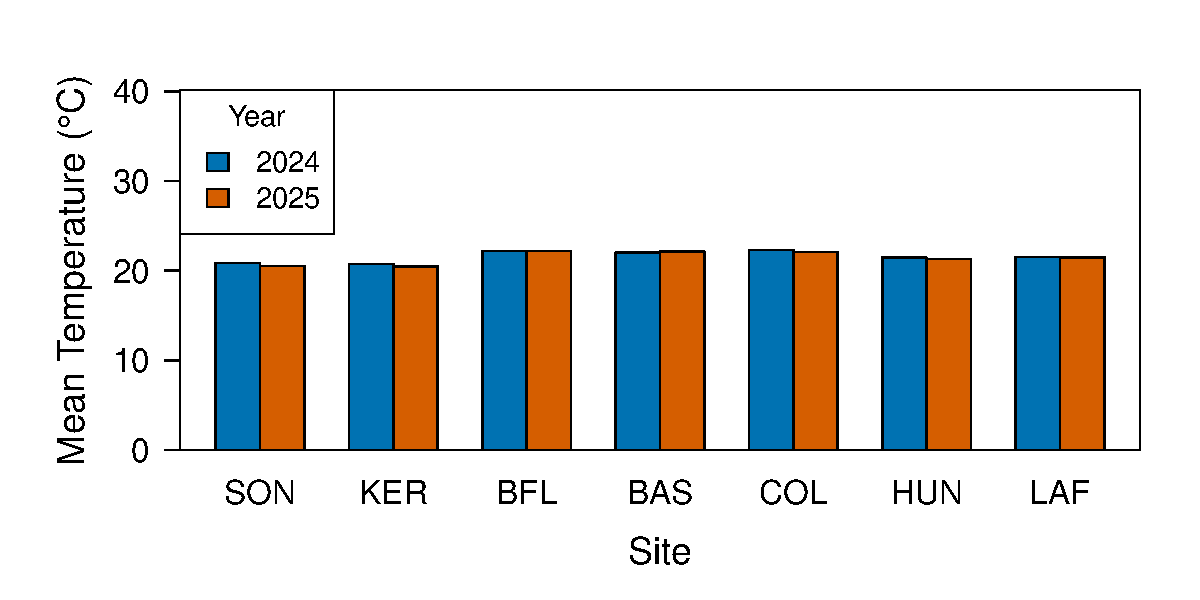
\includegraphics[width=0.8\linewidth]{temp_census_years.pdf}
    \caption{Annual temperature (\degree C) during the 2024 and 2025 census years.
    Sites are arranged west to east by longitude.}
    \label{sup:temp}
\end{figure}
\clearpage

\begin{figure}[ht]
    \centering
    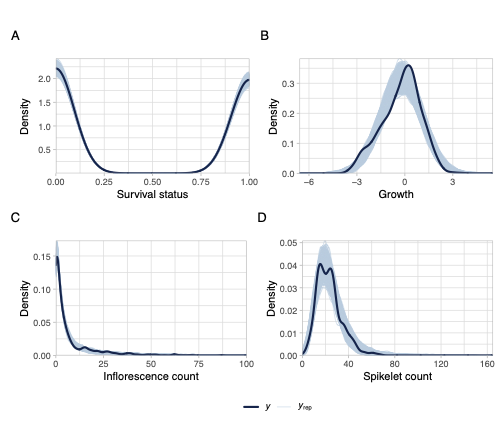
\includegraphics[width=1\textwidth]{PPC.png}
    \caption{Posterior predictive checks for each vital rate.
    Dark blue lines show observed data ($y$) and light blue lines show replicated datasets from posterior predictions ($y_{\text{rep}}$).
    Strong overlap across survival, growth, inflorescence, and spikelet production indicates adequate model fit for all vital rates.}
    \label{sup:ppc_vital}
\end{figure}
\clearpage

\begin{figure}[ht]
    \centering
    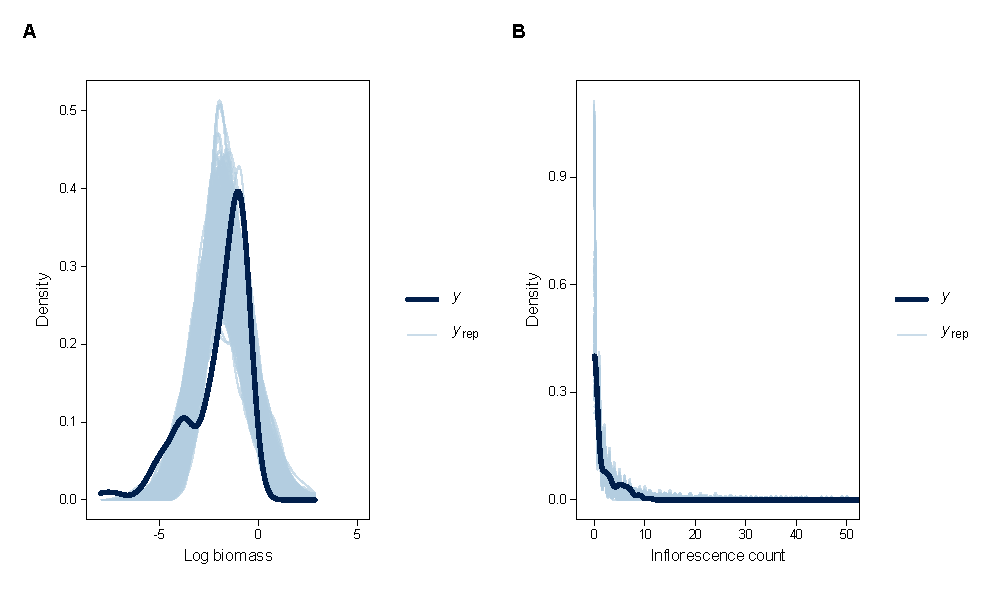
\includegraphics[width=\textwidth]{PPC_models_soilendo.pdf}
    \caption{Posterior predictive checks for Bayesian models of plant performance in the greenhouse experiment.
    Density overlays show observed data (solid line) and 200 posterior predictive draws (shaded lines) for (A) aboveground biomass and
    (B) inflorescence count per plant.
    Models adequately capture the distribution of observed data across all response variables.}
    \label{sup:ppc_models_soil}
\end{figure}
\clearpage


\begin{figure}[ht]
    \centering
    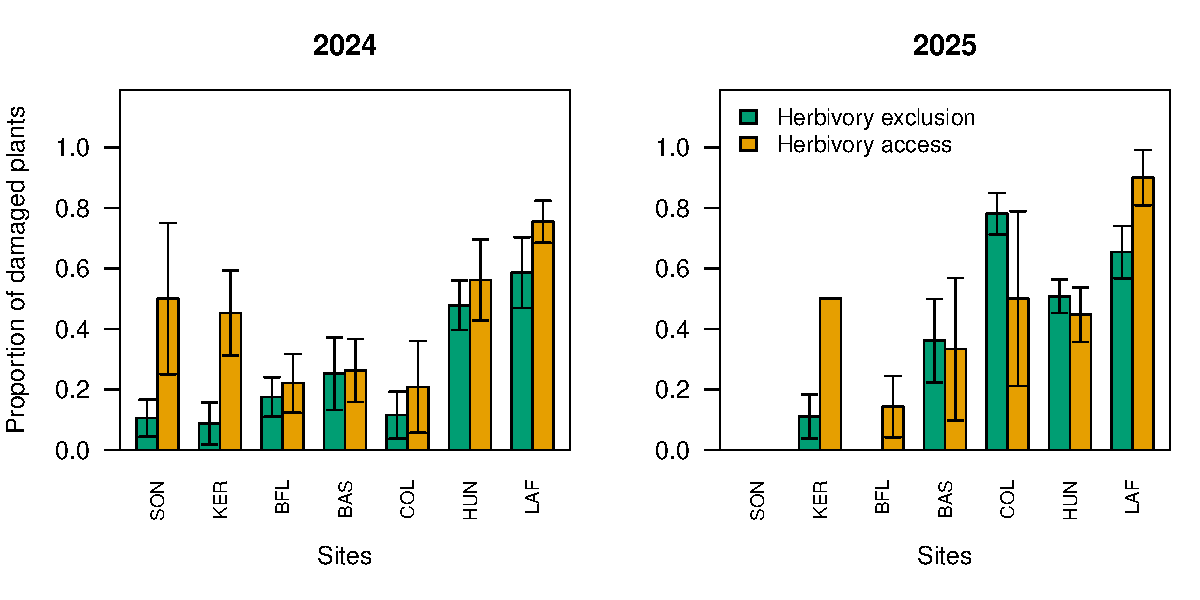
\includegraphics[width=1\linewidth]{prop_damage_barplot_24_25.pdf}
    \caption{Proportion of plants damaged by herbivory across sites in 2024 and 2025.
    Sites are ordered west to east.
    Error bars indicate standard errors across plots within each site.
    Panels show results for 2024 (left) and 2025 (right).}
    \label{sup:herb}
\end{figure}
\clearpage

\begin{figure}[ht]
    \centering
    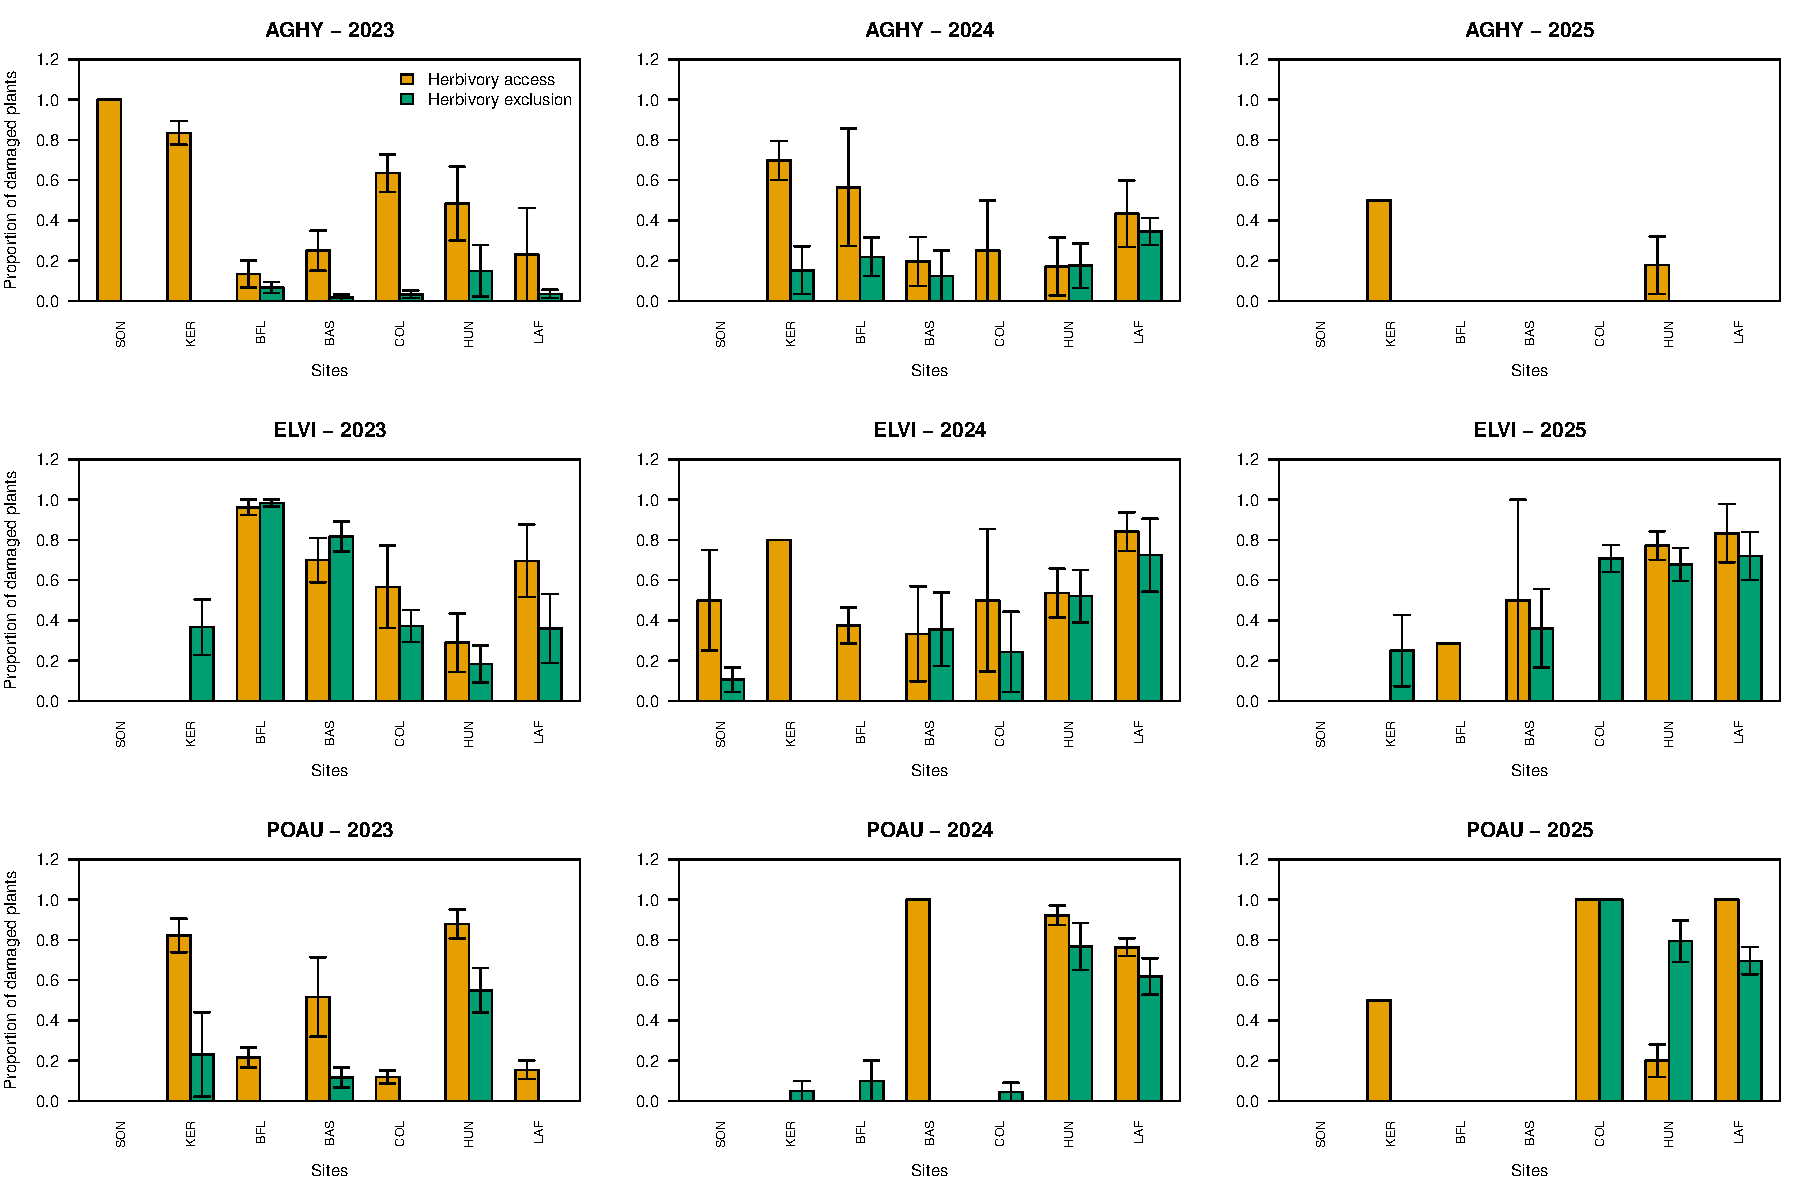
\includegraphics[width=1\linewidth]{prop_damage_species_years.pdf}
    \caption{Proportion of plants damaged by herbivory across sites for
    \textit{Agrostis hyemalis}, \textit{Elymus virginicus}, and
    \textit{Poa autumnalis} over 2023--2025.
    Sites are ordered west to east.
    Error bars indicate standard errors across plots within each site.
    Panels are arranged by species (rows) and year (columns).}
    \label{sup:herbsp}
\end{figure}
\clearpage


\begin{figure}[ht]
\centering
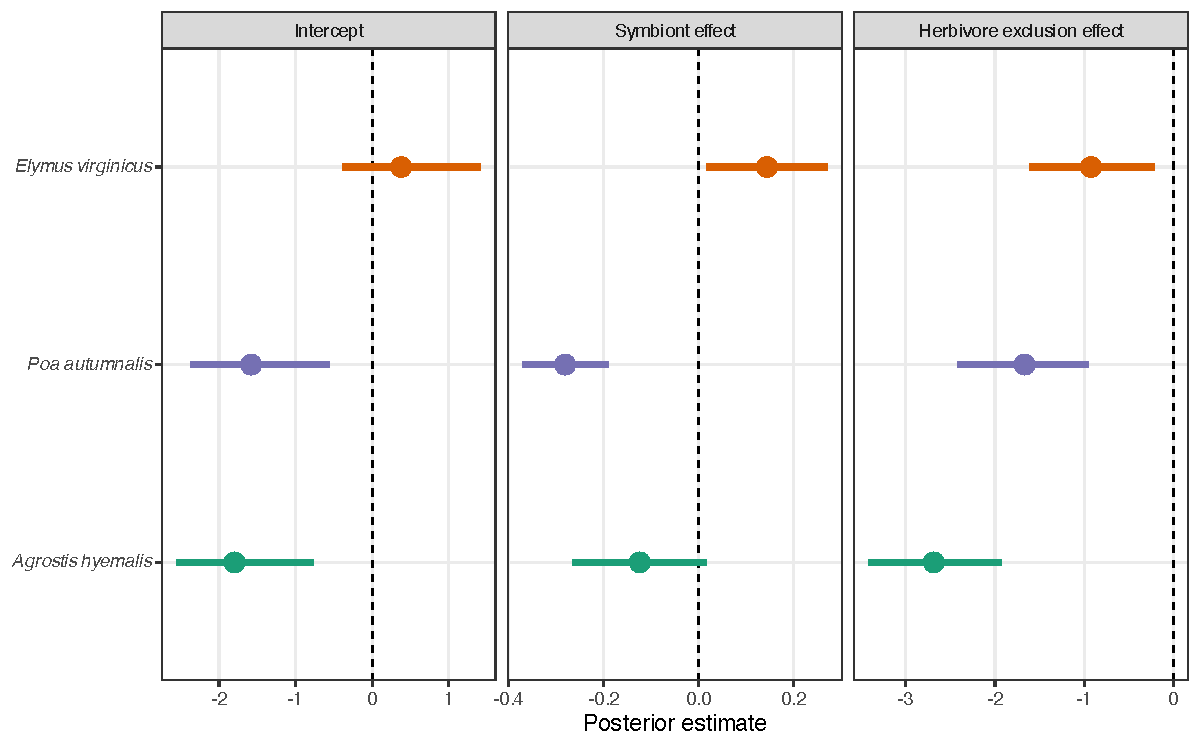
\includegraphics[width=1\linewidth]{herb_endo_effect.pdf}
\caption{Posterior estimates (median and 90\% credible intervals) of symbiont and herbivore exclusion effects on the proportion of damaged tillers for three host grass species, from a binomial model with site, year, and plot as random effects. Negative values indicate reduced herbivore damage, whereas positive values indicate increased damage. Back-transformed to predicted proportions of damaged tillers in herbivore-access plots, symbiosis reduced damage in \textit{P. autumnalis} ($S^+$: 13.5\% vs.\ $S^-$: 17.1\%) and, more weakly, in \textit{A. hyemalis} ($S^+$: 12.8\% vs.\ $S^-$: 14.2\%), and increased damage in \textit{E. virginicus} ($S^+$: 62.8\% vs.\ $S^-$: 59.4\%). Points and intervals are colored by species: \textit{Agrostis hyemalis} (green), \textit{Elymus virginicus} (orange), and \textit{Poa autumnalis} (purple). Dashed vertical lines indicate no effect.}
\label{sup:herbivory}
\end{figure}
\clearpage


\begin{figure}[htp]
\centering
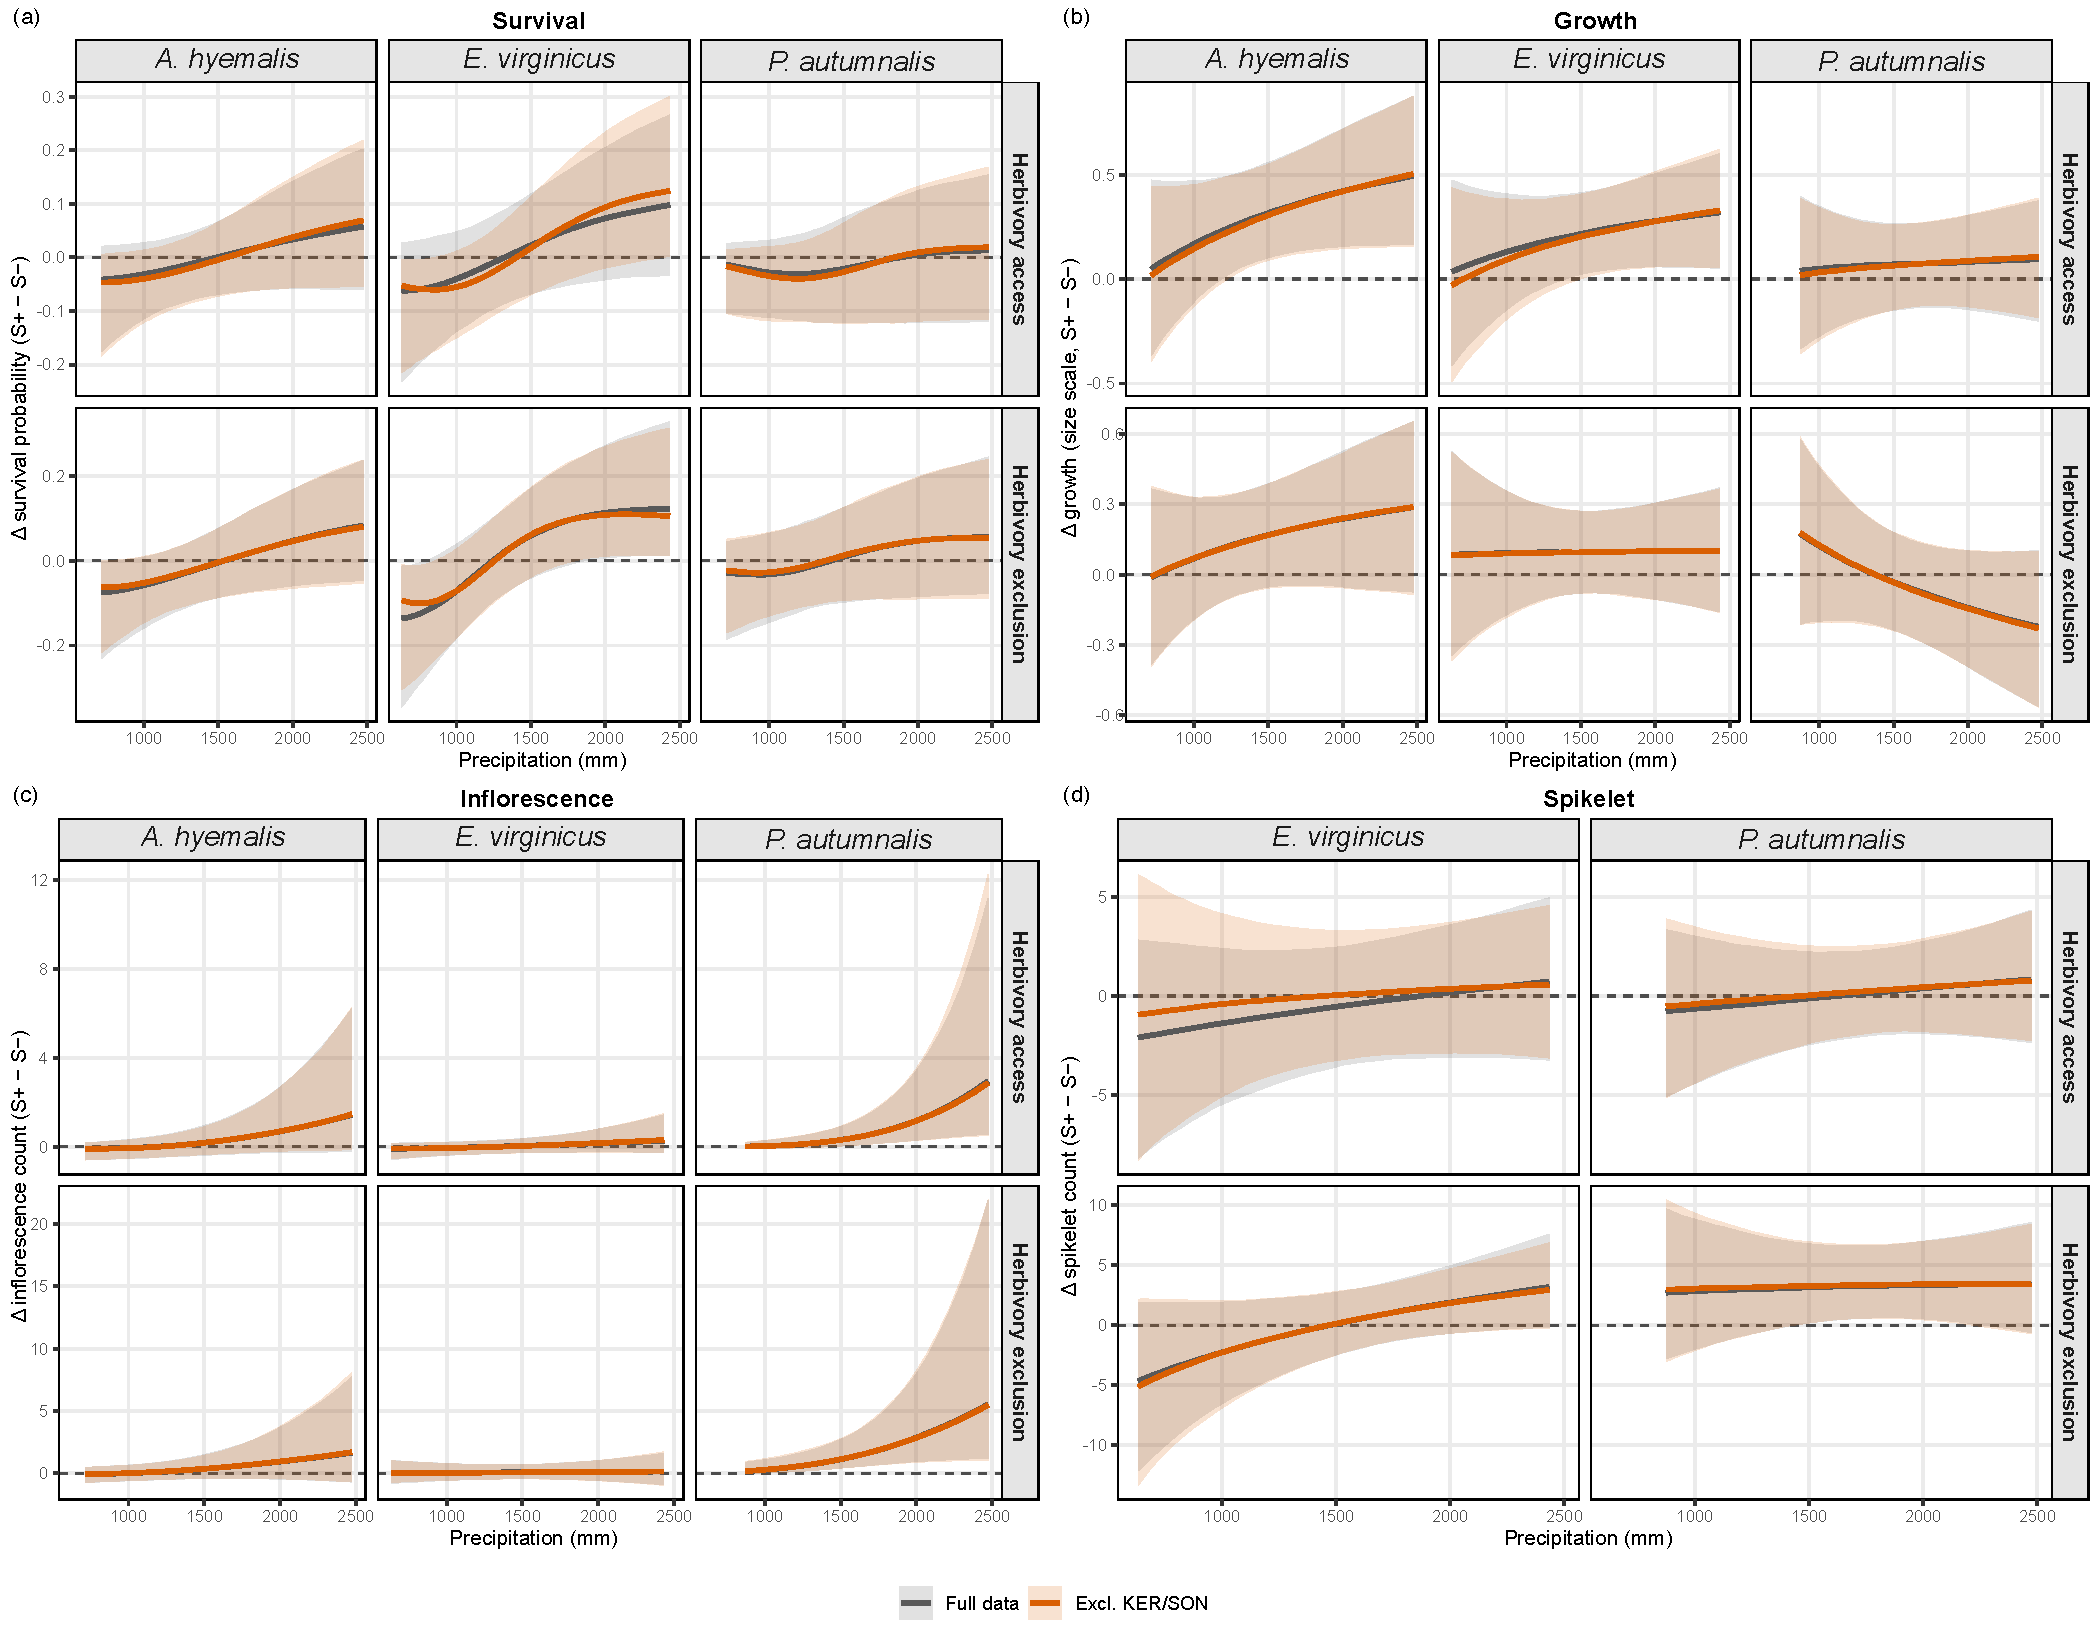
\includegraphics[width=\textwidth]{FigS_sensitivity_KER_SON_combined.pdf}
\caption{Sensitivity of estimated endophyte effects ($\Delta$ = $S^+ - S^-$) on (a) survival, (b) growth, (c) inflorescence production, and (d) spikelet production to exclusion of sites KER and SON, which were destroyed by deer and subsequently replanted in 2024. Lines and shaded bands show posterior median and 90\% credible intervals for the full dataset (gray) and for the dataset excluding KER and SON (orange). Estimated effects were nearly identical between the two datasets across all species, vital rates, and herbivory treatments, indicating that the disturbance and replanting at these sites did not meaningfully influence our conclusions.}
\label{fig:sensitivity_KER_SON}
\end{figure}
\clearpage

\begin{figure}[htp]
    \centering
    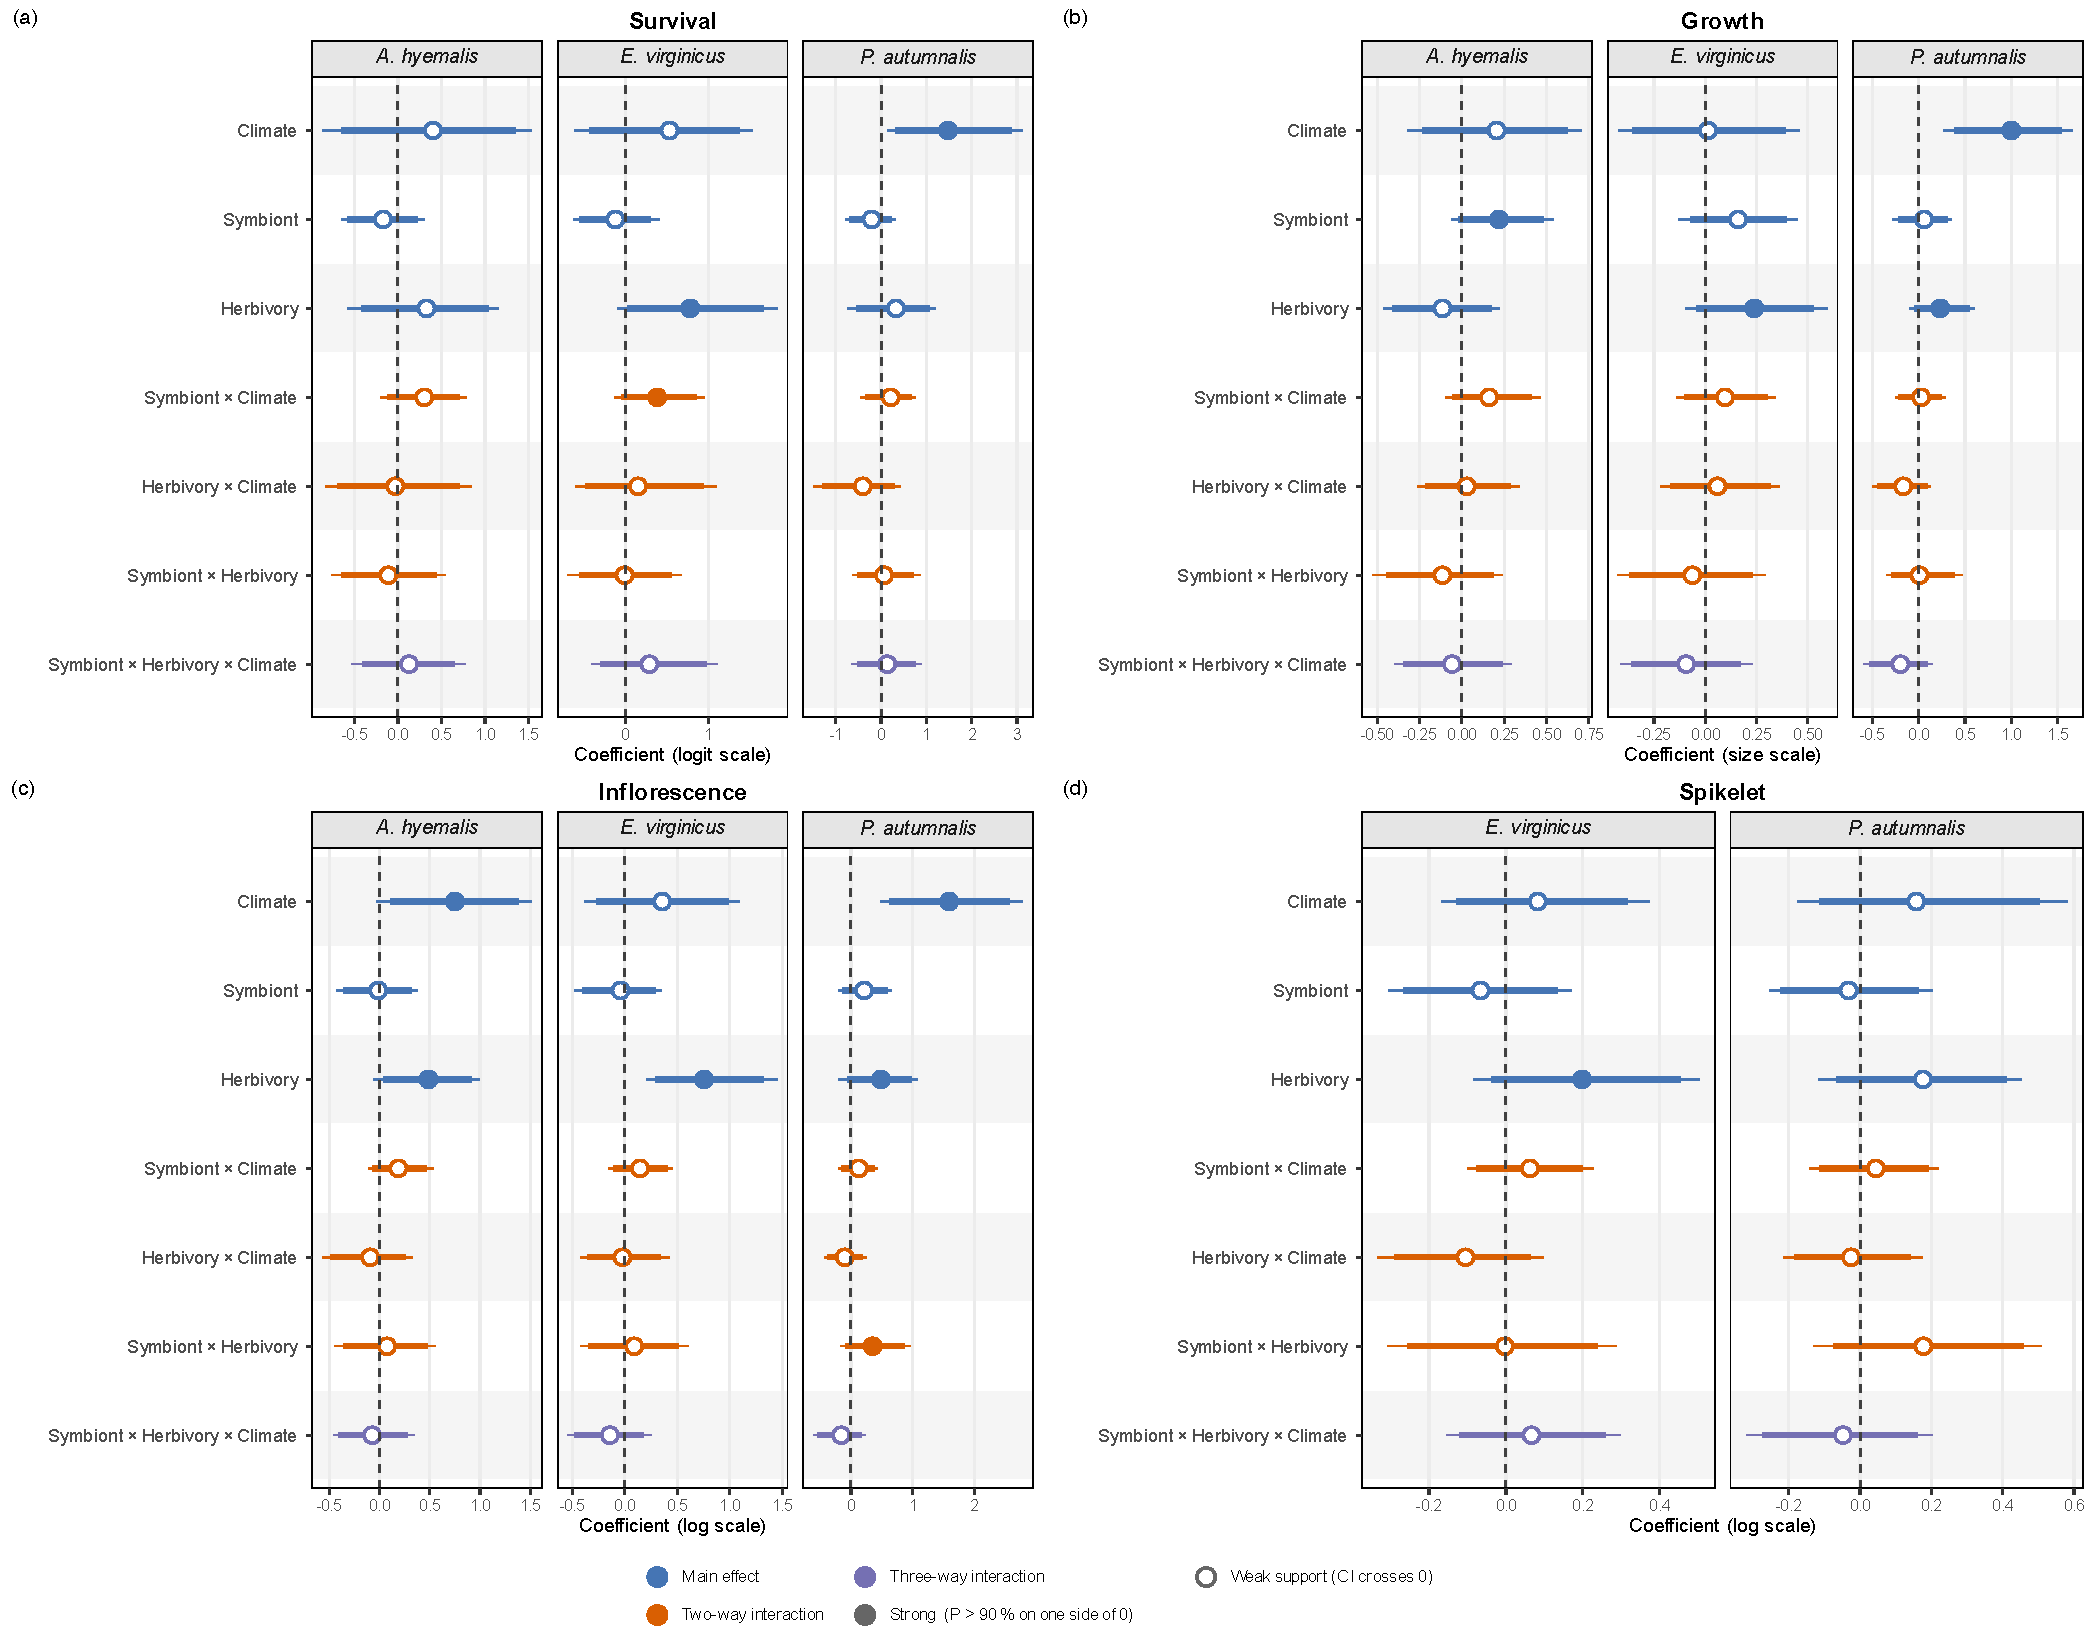
\includegraphics[width=1\textwidth]{FigS_coef_caterpillar_combined.pdf}
    \caption{
Posterior summaries of standardized regression coefficients from Bayesian models of survival, growth, inflorescence production, and spikelet production across three cool-season grass species (\textit{Agrostis hyemalis}, \textit{Elymus virginicus}, and \textit{Poa autumnalis}; spikelet production was modeled for \textit{E. virginicus} and \textit{P. autumnalis} only). 
Panels show median posterior estimates (points), 90\% credible intervals (thick bars), and 95\% credible intervals (thin bars) for main effects of climate (precipitation), endophyte presence, and herbivory, as well as their two-way and three-way interactions. 
Filled points indicate strong posterior support for an effect ($\mathrm{Pr}(\beta > 0)$ or $\mathrm{Pr}(\beta < 0) > 0.90$), whereas open points indicate weaker support. Colors distinguish main effects, two-way interactions, and three-way interactions. Vertical dashed lines indicate no effect ($\beta = 0$). 
Coefficients are shown on the model link scale: logit for survival, linear size scale for growth, and log scale for inflorescence and spikelet production.
}
    \label{sup:coef_caterpillar}
\end{figure}
\clearpage

\begin{figure}[htp]
    \centering
    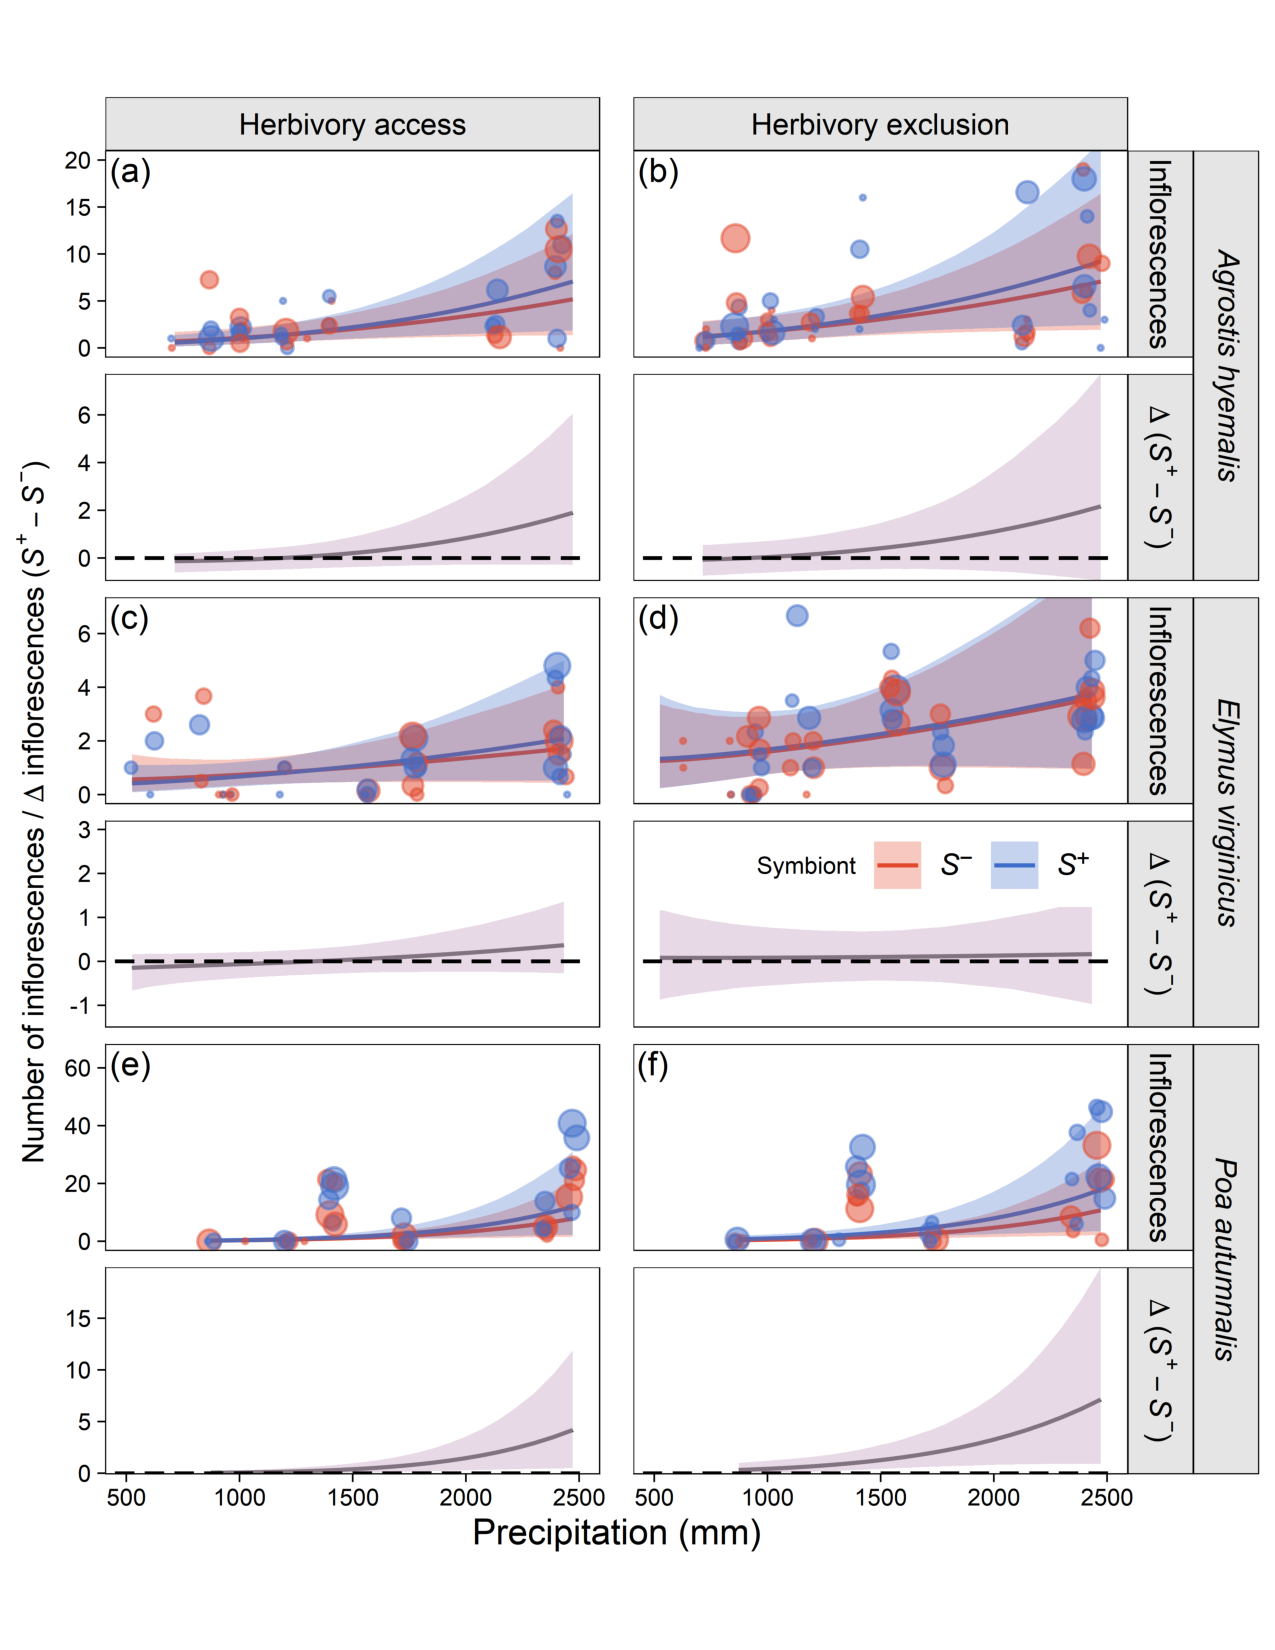
\includegraphics[width=1\textwidth]{Inflorescence_diff_v.pdf}
    \caption{Predicted inflorescence production (upper panels) and symbiont effect ($\Delta$ = $S^+ - S^-$; lower panels) across the precipitation
    gradient.
    Lines show posterior means with 90\% credible intervals.
    Points represent mean observed inflorescences per plot, slightly jittered for visualization.
    The dashed line at $\Delta = 0$ indicates no symbiont effect.
    Panels are arranged by species and herbivory treatment (herbivore access and exclusion).
    All panels share a common x-axis for illustrative purposes; some species extend beyond their observed precipitation range.}
    \label{sup:inflo}
\end{figure}
\clearpage

\begin{figure}[htp]
    \centering
    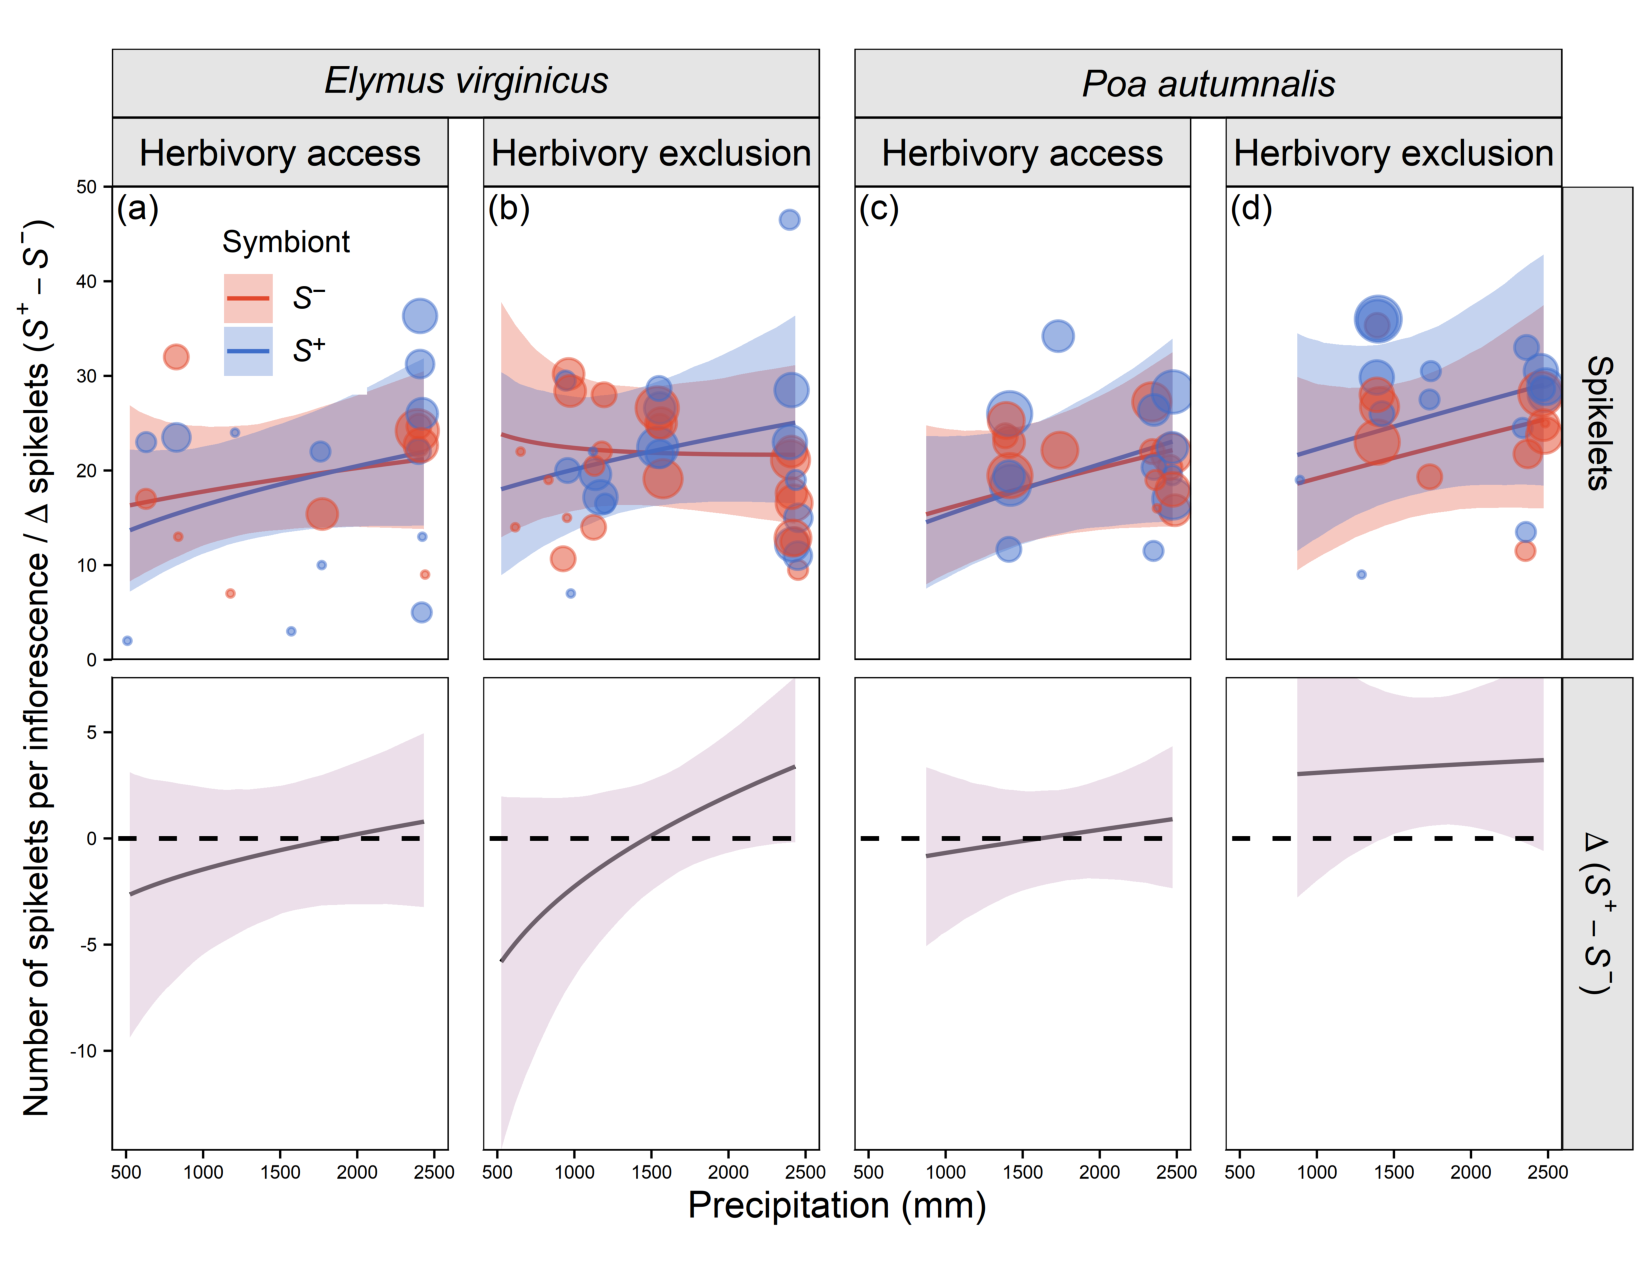
\includegraphics[width=1\textwidth]{Spikelet_diff.pdf}
    \caption{Predicted spikelet production (upper panels) and symbiont effect ($\Delta$ = $S^+ - S^-$; lower panels) across the precipitation
    gradient.
    Lines show posterior means with 90\% credible intervals.
    Points represent mean observed spikelets per plot, slightly jittered for visualization.
    Spikelets were measured for two species only (see Methods).
    The dashed line at $\Delta = 0$ indicates no symbiont effect.
    Panels are arranged by species and herbivory treatment (herbivore access and exclusion).
    All panels share a common x-axis for illustrative purposes; some species extend beyond their observed precipitation range.}
    \label{sup:spikelet}
\end{figure}
\clearpage

\begin{figure}[htp]
    \centering
    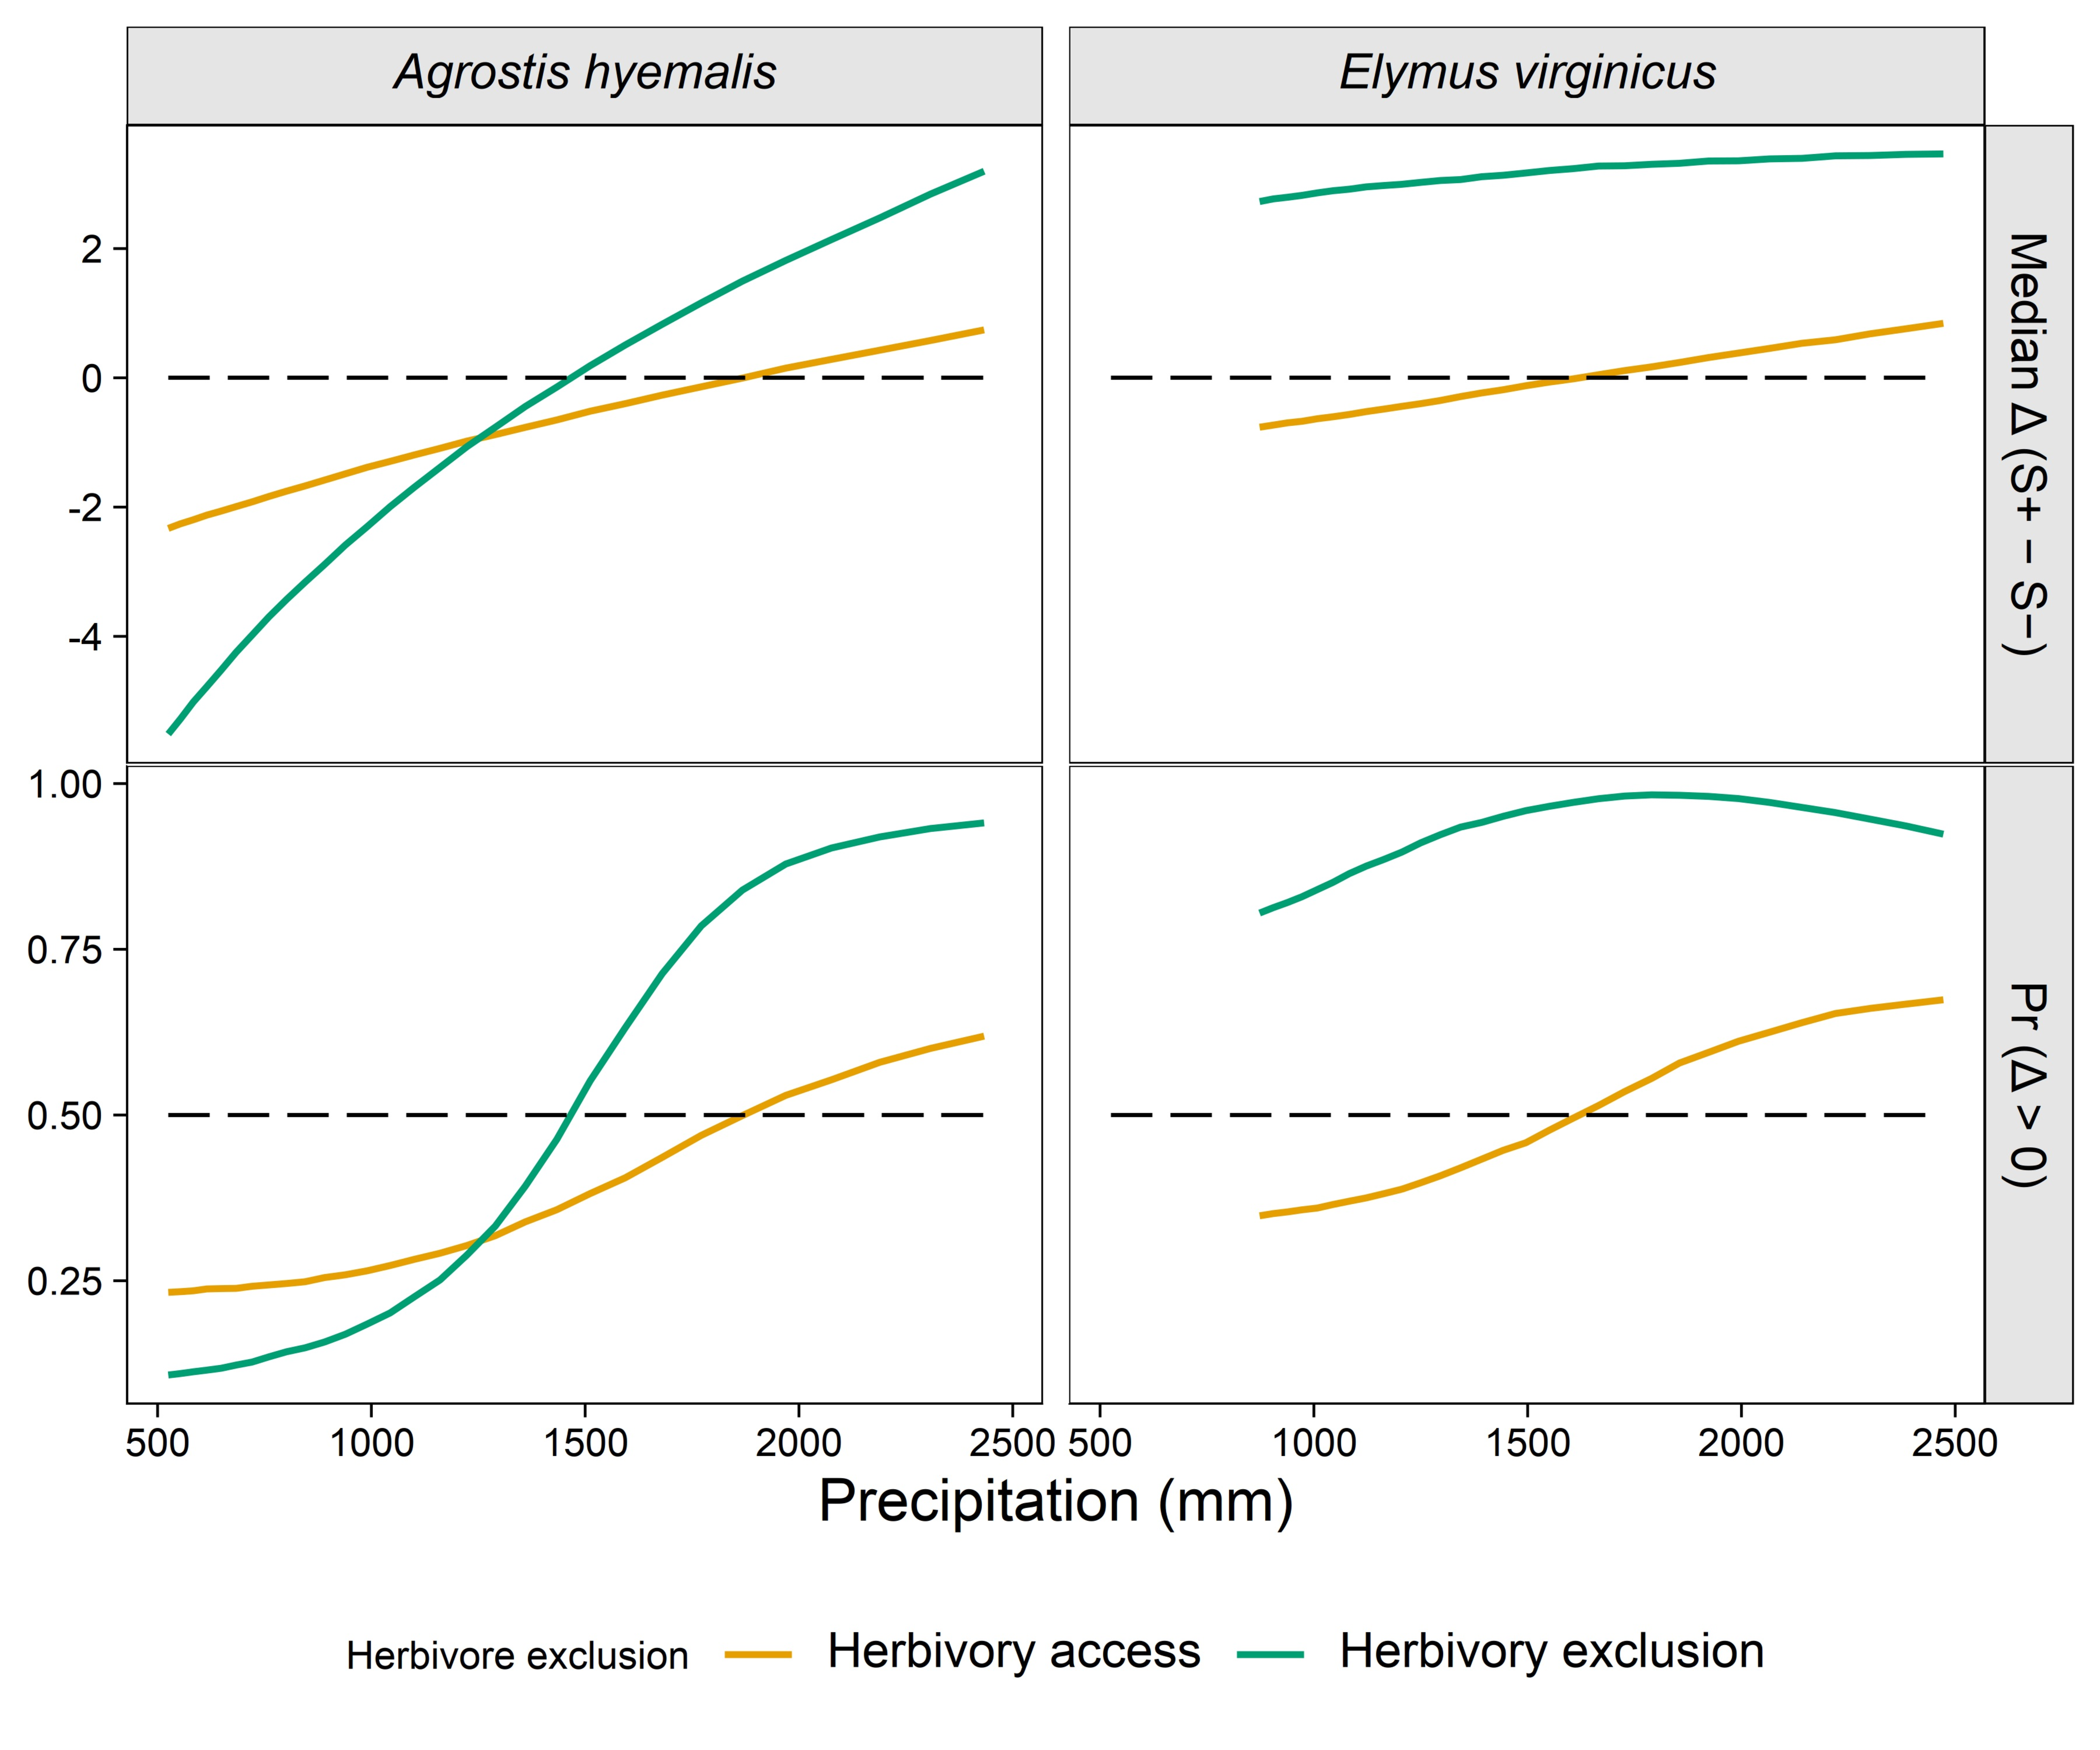
\includegraphics[width=1\linewidth]{Spikelet_diff_stat.pdf}
    \caption{Median $\Delta$ ($S^+ - S^-$) and posterior probability $P(\Delta > 0)$ for spikelet production across precipitation quantiles for each species and herbivory treatment.
    Herbivore exclusion treatments are indicated by colour.
    Horizontal dashed lines indicate $\Delta = 0$ for medians and $P(\Delta > 0) = 0.5$ for probabilities.
    Panels are arranged by metric and species.}
    \label{sup:spike_delta}
\end{figure}
\clearpage

\begin{figure}[htbp]
\centering
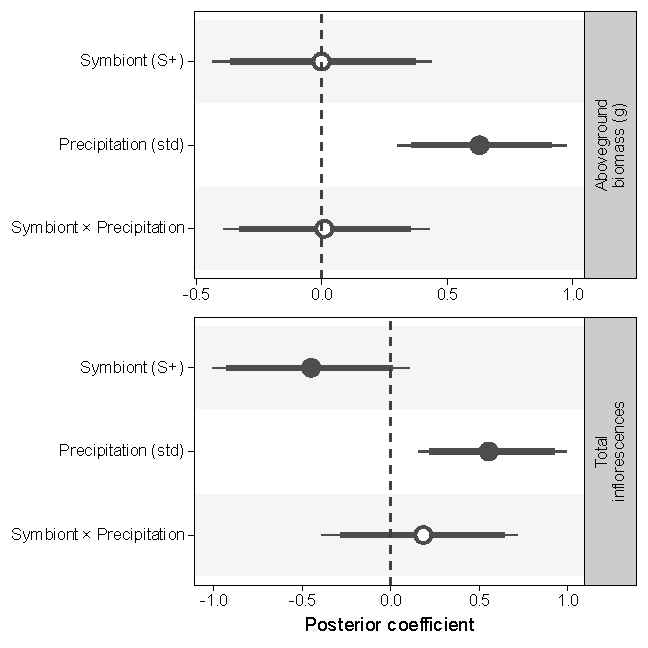
\includegraphics[width=0.6\textwidth]{Fig_Greenhouse_Coefficients.pdf}
\caption{Posterior coefficient estimates for the greenhouse experiment (median, with thick and thin bars showing 90\% and 95\% credible intervals) for symbiont presence, soil-origin precipitation (standardized), and their interaction, for aboveground biomass (top) and total inflorescences (bottom). Filled points indicate estimates with posterior probability $> 0.9$ of being above or below zero; the dashed line marks zero.}
\label{sup:greenhouse_coef}
\end{figure}


\clearpage
\bibliographystyle{apalike}
\bibliography{References}

\end{document}